\documentclass{ctexart}
\usepackage{color}
\usepackage{fancyhdr}
\usepackage[a4paper, left=1in, right=1in, top=1in, bottom=1in]{geometry}
\usepackage{graphicx}

\pagestyle{fancy}
\fancyhf{}
\renewcommand{\headrulewidth}{0pt}
\renewcommand{\footrulewidth}{0pt}
\lhead{完全不一样的Matrix: Reloaded}
\rhead{\thepage}

\definecolor{green}{rgb}{0.0, 0.25, 0.0}
\newcommand{\myparsep}{\noindent \rule[0.5ex]{\linewidth}{1pt}}
\newenvironment{myquote}{\color{green} \setlength{\leftskip}{6em} \setlength{\rightskip}{4em} \setlength{\parindent}{-2em}}{\par}

\hyphenation{ani-ma-trix}

\begin{document}
\centerline{\bf \fontsize{15.75pt} \baselineskip \selectfont The Matrix: Reloaded非官方解释}
\vspace{12pt}
\centerline{作者:neverwin}
\centerline{Version 0.90 2006-08-03}
\centerline{重制:woctordho}
\centerline{2017-02-18}
\vspace{12pt}

完成第一部Matrix的“非官方解释”己经有8个多月了,中间停下来写了一些Matrix专题的分析,不是想偷懒,而是觉得需要一些时间来完成一些关于Matrix的整体的理解。现在neverwin我又回来了,又一次站在路口,再次出发了。

先要说明一些事情,我个人觉得Matrix第一部的“非官方解读”被部分误读了。

比如,我在最后提到的那个“招牌”,fff6b7,很多人觉得很难接受这么晦涩的Matrix,觉得没有必要去纠缠这样的细节。其实,我写这些东西的目的就是一个,要证明Matrix的导演的IQ比我们高出很多。如果你不能承认这点,你就很难低下头来,去思考Matrix深刻的内涵。

如果现在我接着以第一部的解读方式继续下去,自己肯定逃不出耍小聪明的下场。

所以,第二、三部的“非官方解释”我打算用更简单的方式来完成,不再搞“解谜”了,重点将放在解释电影本身的剧情上。

但我要说的是,第二、三部的电影谜题比第一部要多得多、复杂得多,就像一条走不完的路。愿意猜谜的朋友们可以在这个方向上走得更远,有兴趣的也可以私下和我交流,文章结尾有联系方式。

废话够多了,让我们开始吧~

请各位朋友带着一颗谦恭的心,用心来“看”这部伟大的电影作品。

\myparsep

\begin{myquote}
Guard 1: See you tomorrow.

Guard 2: Oh, my God.

Trinity: I'm in.
\end{myquote}

让黑客迷苦等四年的Matrix终于回来了!我却没赶上,不怎么喜欢第一部,就没怎么激动地等着它。也许这就是缘分,注定的东西,你想错过它,却一口被它死死咬住了。

导演兄弟说了,电影开头的绿色动画代表的是整部的故事内容,那我们就试着来解释一下。

\begin{figure}[htb]
\centering
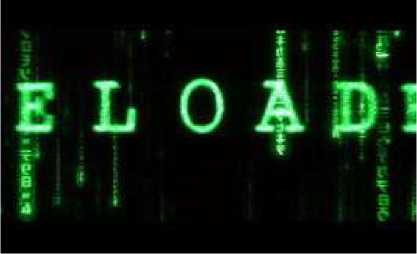
\includegraphics[width=0.5\linewidth]{fig/read_reloaded-1}
\end{figure}

动画是从Reloaded中的O开始的,这个O说起来是一个圆圈,因为第二部说的是the One道路的必然性和重复性,之前版本的the One最后选择救全人类……当然,这集的最后,我们看到这个“圆”被打破。

O也可以看成是0, 还记得处处可见的101吗?除了之前提到的那些解释,我想加一个很重要的,从Architect嘴里套出来的一个解释:1代表的是the One,代表的是系统缺陷,代表的是Matrix更新换代;反之,0代表的就是一个平稳运行的Matrix;所以“101”连起来看就是在两次“系统更新换代”中的Matrix。在第二部里,我们看到的一个很重要的主题是Oracle如何来打破Matrix的平衡性,打破这个0,这就是“零”的另外一个意思。

\begin{figure}[htb]
\centering
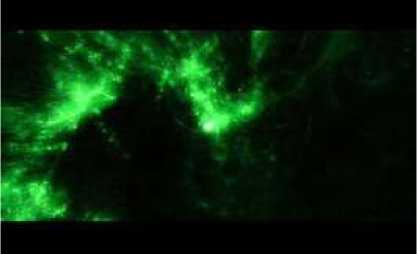
\includegraphics[width=0.5\linewidth]{fig/read_reloaded-2}
\end{figure}

紧接着出现的是我们代表宇宙大爆炸的星云。大爆炸理论也是导演兄弟很推崇的一个理论,简单来说就是讲宇宙的起源来自一次大爆炸,广义上可以扩展到哲学,大乱后方有大治,Matrix需要Oracle的“不平衡”来产生革命性的新秩序。

\begin{figure}[htb]
\centering
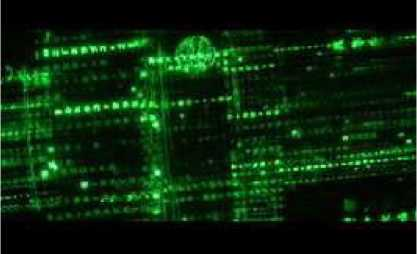
\includegraphics[width=0.5\linewidth]{fig/read_reloaded-3}
\end{figure}

动画的结尾部分是个挂钟的内部结构,转动的齿轮。如果你仔细看,可以看到好几个镜头出现了一个小螺帽,这是在强调系统的复杂性。一个小小的细节却是系统不可缺少的重要部分,就像在Neo的the One之路中,每个人都有它的角色,就算是张卫生纸,也是有它的用途的。

\begin{figure}[htb]
\centering
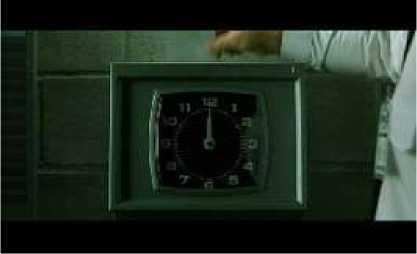
\includegraphics[width=0.5\linewidth]{fig/read_reloaded-4}
\end{figure}

钟所代表的更重要的意思,当然是时间了。这里的时间有好几层意思:

1、Everything that has a beginning has an end. 万事有始有终。看看那个钟,12点~电影开始了,12点既是开始也是结束,电影在这个时刻开始,是在告诉我们,时间己经到了决定是“开始”新的Matrix还是“结束”世界的时候了。

2、就像Trainman在ETM游戏里说的,Neo他们己经没有多少时间了。

3、时间的重要性。在法国人的话里,你们(人类)没有时间,这里没有时间的意思是你们不知道现在到底是什么时候,Zion里的人以为是2199年,其实根本不是。

镜头终于转到了Matrix里,我们看到的是电力公司的那堆警卫在换岗。

一个警卫说:“See you tomorrow.”(明天见)很简单的再见方式,可是在电影里,特别是第二、三部里,明天(tomorrow)指的是“未来”,系统稳定的未来。Oracle说“我怕明天再也不会来了”,她说的明天就是下一代的Matrix。Neo如果失败,下一代的Matrix就得胎死腹中了。

\begin{figure}[htb]
\centering
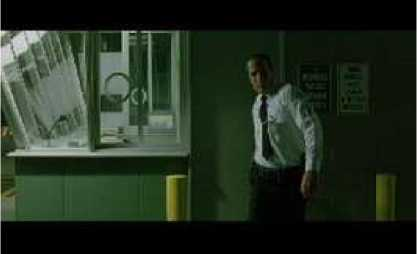
\includegraphics[width=0.5\linewidth]{fig/read_reloaded-5}
\end{figure}

下面这个镜头,警卫走出房间,门口右边的墙上,有两个牌子,一个是黑底白字的“Visitors please return passes”(访客请交还通行证),另外一个是白底黑字的“All truck drivers must remain with their vehicles”(卡车司机不能下车)。

参照我在第一部的非官方解释里提到的黑白色的含义,第一个牌子是黑色的,是写给黑客们看的,这里的pass也可以翻译成路径、道路,整句的意思是说Neo要回到返回Source的道路去。

第二个牌子呢,还记得第二部后面高速公路上那场戏吗?两个干探各开着一辆卡车对撞,他们是不是“卡车司机”啊?两个牌子加起来,实际是在说人和干探程序都被规则所限,一黑一白,跑不掉。

\begin{figure}[htb]
\centering
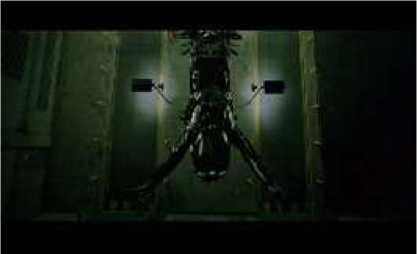
\includegraphics[width=0.5\linewidth]{fig/read_reloaded-6}
\end{figure}

Trinity出场了。先请大家注意,她的出场是她在驾驶摩托车的背影,脑袋盖着头盔,所以,我们第一眼看到的Trinity实际是她的身体。等后面Neo、Morpheus、Smith都出场了,我一起解释这个的含义。

\begin{figure}[htb]
\centering
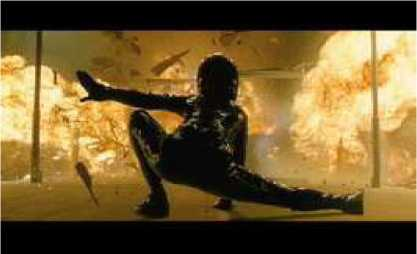
\includegraphics[width=0.5\linewidth]{fig/read_reloaded-7}
\end{figure}

炸掉警卫室的爆炸效果很震撼吧!联系第一部的电梯爆炸,火,代表了革命,代表了对旧事物的革新。这里Trinity摆了个造型,这个造型像什么?大家自己琢磨吧,算是课后的作业。

\begin{figure}[htb]
\centering
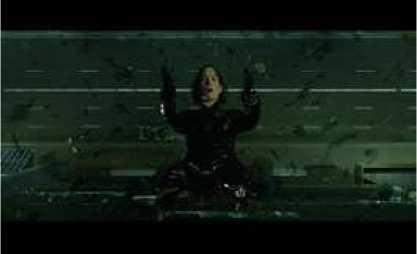
\includegraphics[width=0.5\linewidth]{fig/read_reloaded-9}
\end{figure}

接下去的Trinity中枪的镜头和后面的“真实发生”的场景没有镜头重复。我相当喜欢那个子弹击中Trinity时鲜血溅出的镜头,不是因为我嗜血,而是它让我更深地理解了Trinity为爱牺牲的精神。

\begin{figure}[!htb]
\centering
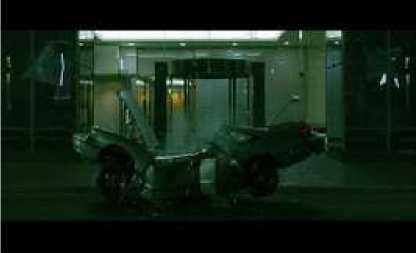
\includegraphics[width=0.5\linewidth]{fig/read_reloaded-10}
\end{figure}

大家注意一下这里Trinity砸中汽车的镜头。后面Neo救了她,这个镜头就被改了,结局也就改了。

\begin{figure}[htb]
\centering
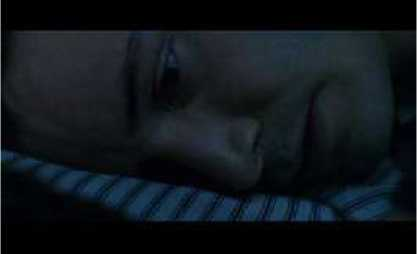
\includegraphics[width=0.5\linewidth]{fig/read_reloaded-11}
\end{figure}

Neo醒来了,我们终于看到了Neo。注意,我们看到的是他的脸,他的头的特写,和Trinity的身体一样,我后面来解释。

\myparsep

\begin{myquote}
Link: Sir, are you sure about this?

Morpheus: I told you, we're going to be all right.

Link: I understand, sir, it's just that ... I'm scoping some serious sentinel activity up here.

Morpheus: Link.

Link: Yes sir?

Morpheus: Given your situation, I can't say I fully understand your reasons for volunteering to operate onboard my ship. However, if you wish to continue to do so, I must ask you to do one thing.

Link: What's that, sir?

Morpheus: To trust me.

Link: Yes, sir, I will, sir ... I mean, I do, sir.

Morpheus: I hope so. Now re-patch the main AC to the hard drives and stand by to broadcast.

Link: Yes, sir.
\end{myquote}

\begin{figure}[htb]
\centering
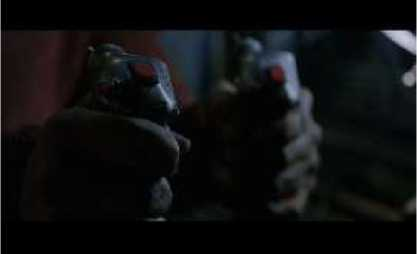
\includegraphics[width=0.5\linewidth]{fig/read_reloaded-12}
\end{figure}

久违的Morpheus也出场了,注意:他先出场的是他在驾驶飞船的手。就差Smith了,我马上要讲它们加起来的含义。

\begin{figure}[htb]
\centering
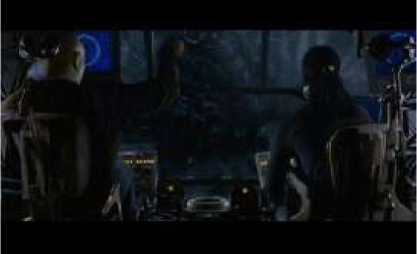
\includegraphics[width=0.5\linewidth]{fig/read_reloaded-13}
\end{figure}

这里还有一个有趣的话题,Morpheus让Link—定要信任他,这一方面是和后面的高速公路追逐时他们的对话对应,另一方面也是在讲述人的理智与机器对抗的一个武器——信任。标准的机器程序眼中只有逻辑和计算,你要一个机器“相信”你,你就得给它一个逻辑上准确的理由。大家如果联系Oracle对Neo的信任,就能明白电影的进行,实际在说明一个很重要的思想:机器和人在互相进化,互相取长补短,新的一代生命体即将诞生。这里不展开,后来再用Sati的例子详细分析。

大家可能都知道了,原来的飞船驾驶员Tank的扮演者因为和导演兄弟吵翻了,也被炒了,剧本被改成Tank死了,他的兄弟Link自愿上了这个飞船。

\begin{myquote}
Trinity: Still can't sleep? You wanna talk?

Neo: They're just dreams.

Trinity: If you're afraid of something ...

Neo: I just wish ... I wish I knew what I'm supposed to do. That's all. I just wish I knew.

Trinity: She's gonna call. Don't worry.

Link: There you are.

Trinity: Are we ready to go?

Link: We' re already late.
\end{myquote}

\begin{figure}[htb]
\centering
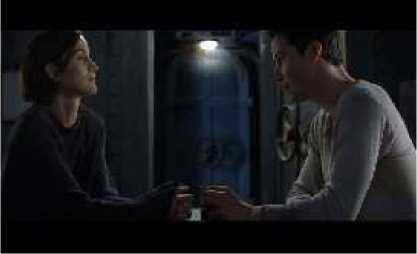
\includegraphics[width=0.5\linewidth]{fig/read_reloaded-14}
\end{figure}

从Trinity问Neo的话中,我们发现Neo最近一直不能入睡,他一直在重复那个可怕的梦。做梦和睡觉变成了两件事,他们在“真实”世界中,“做梦”就等于回到Matrix那个大梦中,此时的Neo和第一部进Oracle厨房的他一样,茫然不知所向。

\myparsep

\begin{myquote}
Niobe: These geotherms confirm the last transmission of the Osiris. The machines are digging. They're boring from the surface straight down to Zion.

Tirant: Mutha ...

Soren: They'll avoid the entire perimeter defense.

Ice: How fast are they moving?

Niobe: Control estimates their descent at a hundred meters an hour.

[Offscreen]: Shit.

[Captain]: How deep are they?

Niobe: Almost two thousand meters.

Tirant: What about the scans from the Osiris?

Ajax: They can't be accurate.

Niobe: They may be.

Ice: What?

Ajax: It's not possible.

Kali: That'd mean there are a quarter of a million sentinels out there.

Niobe: That's right.

Ajax: That can't be.
\end{myquote}

\begin{figure}[htb]
\centering
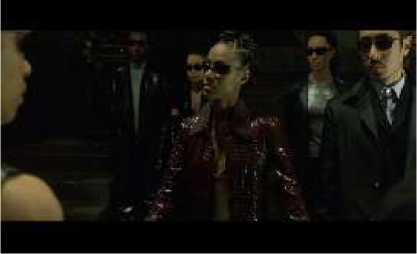
\includegraphics[width=0.5\linewidth]{fig/read_reloaded-15}
\end{figure}

此时在Matrix的一个造船厂中,各个飞船的成员在这里开会,讨论Osiris飞船送来的章鱼大举进攻的消息。Osiris飞船的故事在AniMatrix里有,就是那个老黑和有点像韩国女人比武的那部。最后飞船被章鱼干掉,飞船成员都挂了,电影里的消息就是那个女的冒死在Matrix里的—个信箱里丢下的。后来Niobe他们在Matrix里打了好几架,才抢到这个东西(ETM游戏里的情节)。

25万只章鱼进攻Zion,也恰恰是Zion的人口数目。

\begin{myquote}
Morpheus: Why not? A sentinel for every man, woman, and child in Zion. That sounds exactly like the thinking of a machine to me.

Niobe: Morpheus, glad you could join us.

Morpheus: Niobe. My apologies to all. As you are undoubtedly aware, it has become increasingly difficult to locate a secure broadcast position.

Vector: Squiddies got all our best spots.

Ice: Mainlines are crawling with them.

Ghost: And if Niobe's right, in 72 hours there's gonna be a quarter of a million more.

Ballard: What are we gonna do about it?

Niobe: We' re gonna do what Commander Lock ordered us to do. We'll evacuate broadcast level and return to Zion.

Morpheus: And does the Commander have a plan for stopping 250, 000 sentinels?

Niobe: A strategy is still being formulated.

Morpheus: I'm sure it is.
\end{myquote}

\begin{figure}[htb]
\centering
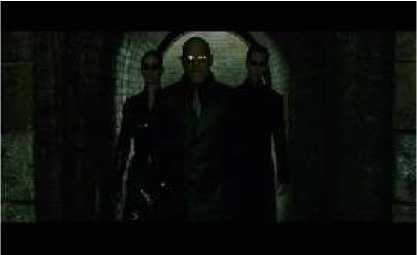
\includegraphics[width=0.5\linewidth]{fig/read_reloaded-16}
\end{figure}

正当大伙儿七嘴八舌,群龙无首时,Morpheus带着他那三人耍酷小团伙出现了。

72个小时,就是3天啊,机器又用3来搞怪了。

这里Morpheus问Niobe,指挥官Lock有啥办法。Niobe说,还在formulate(计划、运算)中。Morpheus很不屑地说,这我也知道。他的意思是,你靠运算能算得过我们的敌人机器程序吗?

\begin{myquote}
[Offscreen]: What do you think we should do, Morpheus?

Morpheus: I think we should proceed as ordered, however ...

Trinity: What is it?

Neo: I don't know.

Morpheus: I must ask one of you for help. Some of you believe as I believe. Some of you do not. But those of you that do, know we are nearing the end of our struggle. The prophecy will be fulfilled soon, but before it can be, the Oracle must be consulted.

Morpheus: If we return and recharge now, we can be back with inside 36 hours. Well before the machines have reached this depth.

Niobe: Do you understand what you' re asking?

Morpheus: I am asking that one ship remain here in our place just in case that the Oracle should attempt to contact us.

Ballard: Bullshit, you're asking for one of us to disobey a direct order.

Morpheus: That's right, I am. But we well know that the reason most of us are here is because of our affinity for disobedience.

Roland: And what happens when you get back to Zion and the Commander throws you in the stockade?

Morpheus: He won't.

Ballard: God damn it, Morpheus, you ain't never gonna change. Shit, I'll do it, just to see what Deadbolt does to you. You got 36 hours.
\end{myquote}

Morpheus此时还深信不疑战争即将结束,很喜欢他的一句话:“我们能在这里都是因为我们天生不听话。”God damn it,它又回来了,看过第一部解释的朋友没有忘吧。

\myparsep

\begin{figure}[htb]
\centering
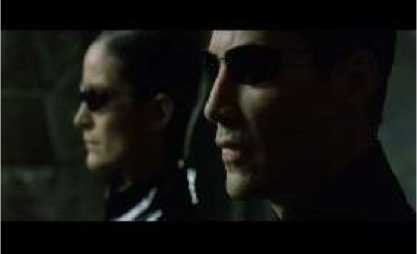
\includegraphics[width=0.5\linewidth]{fig/read_reloaded-17}
\end{figure}

\begin{myquote}
Smith: I'm looking for Neo.

Corrupt: Never heard of him.

Smith: I have something for him. A gift. You see, he set me free.

Corrupt: Fine, whatever. Now piss off.

Neo: Who was that?

Wurm: How did you know someone was here?

Corrupt: He gave you this. He said you set him free.

Wurm: Is everything all right, sir?

Neo: The meeting is over, retreat to your exits. Agents are coming.

Corrupt: Agents?

Neo: Go.
\end{myquote}

从这里开始,每次Smith接近,Neo似乎都有“预感”,起码电影镜头是这样切的,导演是在传递他们之间的联系的信息,后面他们单挑时,我再来说他们的“联系”哈。

Smith来了,先说他的那个奥迪车的车牌,“IS5416”。圣经里的Isaiah 54:16是:“See, it is I who created the blacksmith who fans the coals into flame and forges a weapon fit for its work. And it is I who have created the destroyer to wreak havoc.”他在这里被形容成了制造大破坏的帮手,往后看,是不是很贴切呢?

\begin{figure}[htb]
\centering
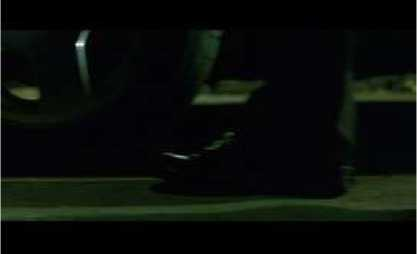
\includegraphics[width=0.5\linewidth]{fig/read_reloaded-18}
\end{figure}

来说个有趣的,前面一直欠着的,我们看到了Smith最先出现的是什么?没错,他的脚。加上前面Trinity的身体 、Neo的脑袋、Morpheus的手。再加上这张可能大家都不陌生的“电影”海报(Zion archive里地铁站里的)——Burly Man.

\begin{figure}[htb]
\centering
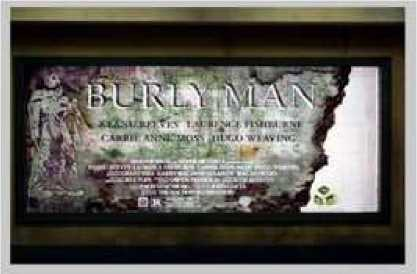
\includegraphics[width=0.5\linewidth]{fig/read_reloaded-19}
\end{figure}

把这些杂碎加起来,是不是一个完整的人?这个组合实际完成了Matrix的革命。Neo的脑袋,不用解释,代表了思想,它是在不断理解学习从而明白自己的义务的。Morpheus的手,手是人认识、改造世界相当重要的部分,它代表的是一种创新的精神。Morpheus相信别人不相信的,做别人觉得不可能做到的事。Trinity的身体,它既是代表了手和脑袋的联系,也是对人的思想的一种支持,人死了脑子还能想吗?Smith的脚,哈,如果你看完三集,还不能理解Neo所到的“境界”是Smith—步一步“带着”他走完的吗?这个脚是指引方向的意思。

这个“人”,这个四人帮,在导演Architect和Oracle的巧妙安排下,完成了Matrix的革命。

\begin{figure}[htb]
\centering
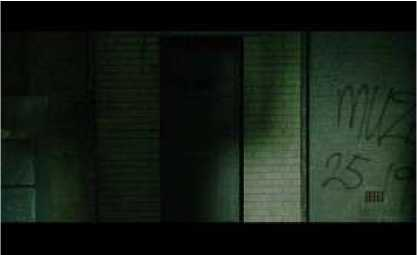
\includegraphics[width=0.5\linewidth]{fig/read_reloaded-20}
\end{figure}

大家注意门的右边墙上写的是“MUZI 25 19”,后面对比Neo放屁前的背景来看。

\begin{figure}[htb]
\centering
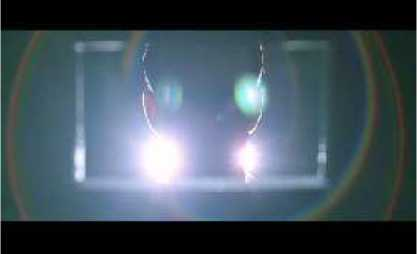
\includegraphics[width=0.5\linewidth]{fig/read_reloaded-21}
\end{figure}

Smith交出耳机,是在宣布他现在不听“上面”发号施令了。他说他自由了,真的吗?我们后面来详细讨论这个问题。

\begin{myquote}
Neo: Hiya, fellas.

Agent Johnson: It's him.

Agent Thompson: The Anomaly.

Agent Jackson: Do we proceed?

Agent Thompson: Yes.

Agent Jackson: He is still ...

Agent Johnson: ... only human.

Neo: Hmm. Upgrades.
\end{myquote}

\begin{figure}[htb]
\centering
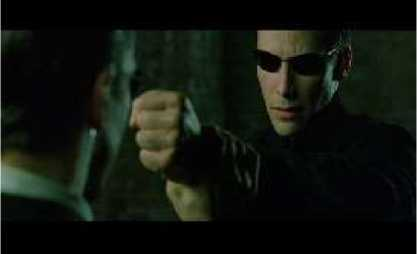
\includegraphics[width=0.5\linewidth]{fig/read_reloaded-22}
\end{figure}

干探来了,可是他们完全不是Neo的对手了,这里Neo说的upgrades(升级了)曾经被很多人提起来讨论,其实很简单,联系画面来看,Neo之前都是单手对付干探,他出另外一只闲着的手要干掉对方时,居然被干探“接招”了。第一部最后,Neo干掉Smith就是单手挡了很多招,最后一脚踢飞了Smith。所以Neo说,机器升级了agent的程序,他们更能打了。

注意到了,干探们一直在强调,Neo还是人。为什么呢?因为程序怕程序,不怕人吗?留到后面来详细讨论。

\begin{myquote}
Smith 1: That went as expected.

Smith 2: Yes.

Smith 1: It's happening exactly as before.

Smith 2: Well, not exactly.
\end{myquote}

\begin{figure}[htb]
\centering
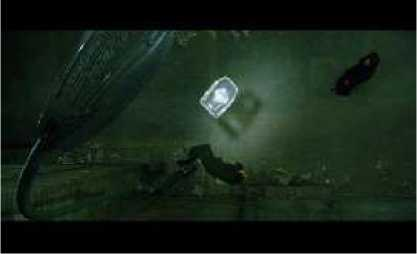
\includegraphics[width=0.5\linewidth]{fig/read_reloaded-23}
\end{figure}

Neo最后一脚把干探踢到灯柱上,灯罩掉了下来,粉碎。灯罩,顾名思义,保护灯泡的东西,保护光,光代表机器的控制,那……明白了吧。

\begin{figure}[htb]
\centering
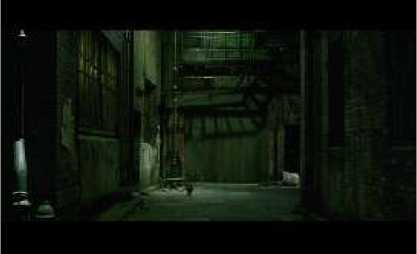
\includegraphics[width=0.5\linewidth]{fig/read_reloaded-24}
\end{figure}

墙角飞起了旧报纸,旧报纸,代表的是旧的信息,就是废弃的程序,那……不就是Smith吗~

\begin{figure}[htb]
\centering
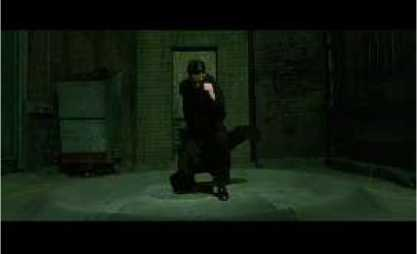
\includegraphics[width=0.5\linewidth]{fig/read_reloaded-25}
\end{figure}

Neo飞起来前,我们看到后面的墙上,之前有“MUZI”的地方被涂掉了……大家发挥自己的想象力吧,哈。

\begin{figure}[htb]
\centering
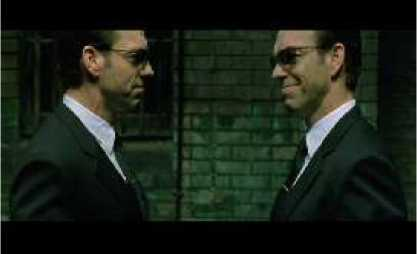
\includegraphics[width=0.5\linewidth]{fig/read_reloaded-26}
\end{figure}

左边的Smith说“完全一样”,右边的说“不完全一样”,左右之分,non-right和right之分。还记得Neo选择的那两个门吗?选择左边的就和以前“完全一样”了,选择右边的就……

\myparsep

\begin{myquote}
Morpheus: What happened back there, Link?

Link: I can't figure it out, sir. Agents just came out of nowhere. And then the code got all weird. Encryption I've never seen.

Trinity: Is Neo okay?

Link: Okay? Shit, Morpheus, you should have seen him.

Morpheus: Where is he now?

Link: He's doing his Superman thing.

Neo: Where are you?
\end{myquote}

\begin{figure}[htb]
\centering
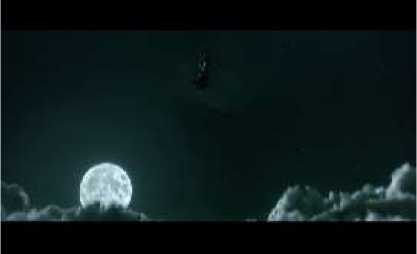
\includegraphics[width=0.5\linewidth]{fig/read_reloaded-27}
\end{figure}

Neo在月光下飞向Oracle的家,因为他有太多问题要问Oracle了。电影里有两次给出了他飞过云层的镜头,第二次在第三部,飞过“真实的”云层,无比美丽的太阳,可是那时的他己经瞎了。他可以看到Matrix里假的月光,却不能看到真实世界里的阳光。你替他难过了吗?不用,他就是来当耶稣的,他注定要受最多的苦。

\begin{figure}[htb]
\centering
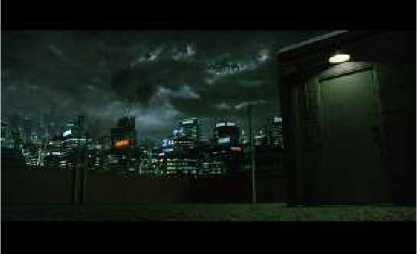
\includegraphics[width=0.5\linewidth]{fig/read_reloaded-28}
\end{figure}

他没走电梯,从楼顶“降落”,那个门上有盏小灯,光正好盖住了整个门。

\begin{figure}[htb]
\centering
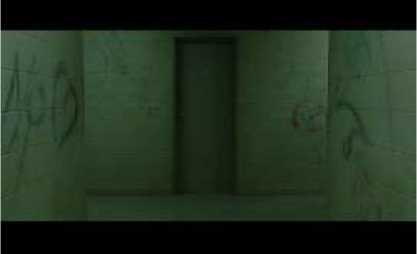
\includegraphics[width=0.5\linewidth]{fig/read_reloaded-29}
\end{figure}

Oracle家门前的走廊是个很有“内容”的地方。首先,整个布局是个“T”,Trinity的T, 三方合作,三位一体,后面找机会详细说这个三位一体。

其次,她的门口的墙上,有很多“涂鸦”。我随便举两个吧:左边的墙上有“No 心形”的符号,在说选左边就没有爱情啦;门的右边有个残缺的圆圈,代表选择右边,the One道路循环的那个圈要被打破。

Oracle不在,你想过吗,为什么不在,因为有人追杀她?不对,如果Oracle在Neo找到前被Smith干掉了,世界不是完蛋了?Oracle—直“掌握”着一切,所以Oracle不是不能见Neo, 而是Neo没有到可以见她的时候,谁决定的? 回头看墙上的牌子吧——Oracle语录,Neo自己决定的。

往后想想,Neo从这之后到见到Oracle之前,他干了什么?干了……什么?

Oracle是要Neo回Zion“休息”一下~为什么呢?大家好好想想吧。等他们回了Zion,我再讨论这个。

\begin{figure}[htb]
\centering
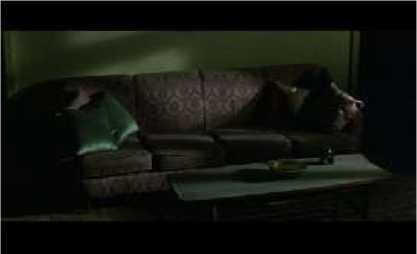
\includegraphics[width=0.5\linewidth]{fig/read_reloaded-30}
\end{figure}

Oracle的房间,摆设都是有讲究的。抓个简单的来说,第三部里Oracle说她要干什么?Unbalance(破坏平衡)。大家看她的沙发垫子,颜色和数量上都是“不平衡”的。

\myparsep

\begin{myquote}
Link: This is the Nebuchadnezzar on approach, requesting access to Gate 3.

Zion Virtual Control Operator: Nebuchadnezzar, this is Zion Control. Maintain present velocity and stand by.

Link: Roger that, Control.

Zion Virtual Control Operator: This is Zion Control requesting immediate stand down of arms at Gate 3. We have the Nebuchadnezzar on approach. Let's open her up. Nebuchadnezzar, you are clear through Gate 3 to Bay 7.

Link: Roger that, Control.

Zion Virtual Control Operator: Door's open. Bed's made. Welcome home.

Link: No place like it.
\end{myquote}

Nebuchadnezzar飞船终于要回Zion了,之前不少人讨论过这个问题:他们是救出Neo后第一次回Zion吗?当然不是,Link不会是用其他飞船送来的吧。

它通过“3号门”到“7号船坞”,通过神奇数字“3”来达到“7”代的Matrix。

大家可能注意到了,这里的指挥塔的操作员也是通过类似接入Matrix的方式,来“虚拟”控制飞船,为什么呢?

\begin{figure}[htb]
\centering
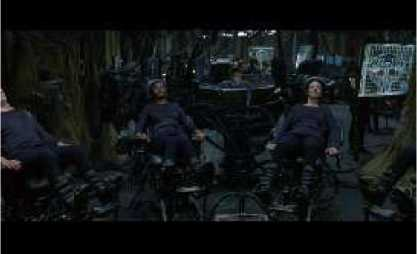
\includegraphics[width=0.5\linewidth]{fig/read_reloaded-31}
\end{figure}

\begin{figure}[htb]
\centering
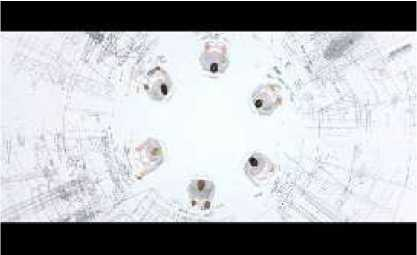
\includegraphics[width=0.5\linewidth]{fig/read_reloaded-32}
\end{figure}

答案很简单,人“醒”的时候不如“睡”的时候好用,这也是在说明人和机器的结合比两个个体单独的作用都大得多。人和机器的结合体,这一进化过程的必然性显现无疑。

那个女控制员说什么了?“Door’s open. Bed’s made. Welcome home.”(门开了,床铺好了,欢迎回家。)

\begin{figure}[htb]
\centering
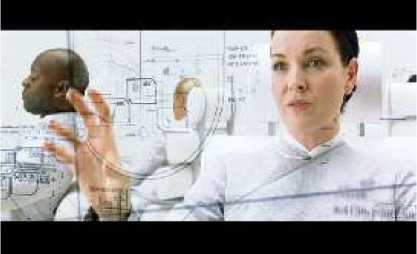
\includegraphics[width=0.5\linewidth]{fig/read_reloaded-33}
\end{figure}

“门开了”——门打开的时候,大家可以回忆一下,后面Oracle说到Neo回Source的场景:“the door full of light”(光芒之门)。Zion的门是不是也有这种感觉呢?动画片里那个小女孩回家时看到的是一道强光源,Source是充满了光的。

\begin{figure}[htb]
\centering
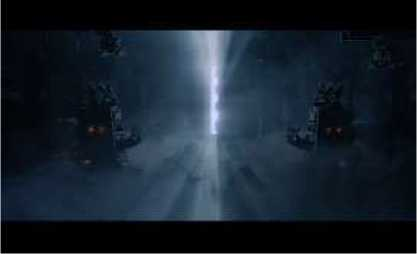
\includegraphics[width=0.5\linewidth]{fig/read_reloaded-34}
\end{figure}

“床铺好了”——赶快带着你上幼儿园的小侄子离开电影院吧,人家都告诉你“床戏”要来了……

\myparsep

\begin{myquote}
Zion Controller: Roger that, Control. Zion Control, stand by for Gate 3 lockdown.

Zion Virtual Control Operator: The Nebuchadnezzar is down. Bay 7.

Zion Controller: Understood.

Morpheus: Captain Mifune.

Mifune: Captain Morpheus.

Morpheus: Are you here to escort me to the stockade, Captain?

Mifune: I'm just here to keep the peace.

A. P. U. Escort: Commander Lock demands ...

Mifune: [coughs]

A. P. U. Escort: ... requests your immediate counsel, sir.

Morpheus: Link.

Link: Sir?

Morpheus: I want the ship ready to go as soon as humanly possible.

Link: Understood, sir.
\end{myquote}

Stockade在流传的盗版翻译中被译成“小黑屋”,实在太贴切了。猫扑己经改变了整整一……大撮人的生活。

\begin{myquote}
Neo: What is it between them?

Trinity: Morpheus and Lock? Niobe.

Neo: Captain Niobe?

Trinity: She used to be with Morpheus. Now she's with Lock.

Neo: What happened?

Trinity: Morpheus went to the Oracle. After that everything changed.

Neo: Yeah, she can do that.

Kid: Neo!

Neo: Oh, no.

Trinity: How does he always know?

Neo: Doesn't he have anything better to do?

Trinity: You know what they say about the life you save.

Neo: I didn't save his life.

Kid: Hiya, Neo! Trinity. Link. It's great to have you back!

Neo: Thanks. It's good to be back.

Kid: Can I carry that for you, Neo?

Neo: No, I can carry my own bag.

Kid: Trinity?

Trinity: I'm fine.

Link: You can carry these.

Kid: Yeah, sure, Link. Hey, you know, next year I'm old enough to join a crew. I've been thinking a lot about it and I've made my decision.

Link: Let me guess.

Kid: I want to join the Nebuchadnezzar. I know Morpheus hasn't filled the other crew positions except for you, Link. I'm sure he has his reasons, but the more I think about it, the more I think it's meant to be. You know, it's fate. I mean, you' re the reason I'm here, Neo.

Neo: I told you, Kid, you found me, I didn't find you.

Kid: I know, but you got me out! You saved me!

Neo: You saved yourself.
\end{myquote}

\begin{figure}[htb]
\centering
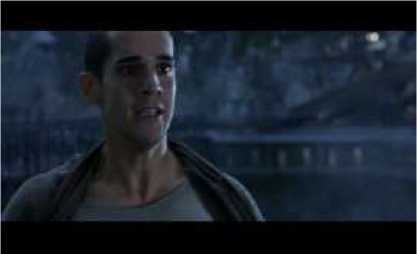
\includegraphics[width=0.5\linewidth]{fig/read_reloaded-35}
\end{figure}

Kid的故事,在Animatrix里详细介绍了。给那些没看过动画片的朋友稍微介绍一下:他也是电脑黑客,中学生,他一直在寻找“答案”,直到他找到了Neo。他用自杀的方式来脱离Matrix(比Neo吃药的方式更加高级)。Kid虽然自杀,可是他的mind(思想)坚信自己没死,只是要从Matrix中醒来,这就是他比Neo更牛的地方。

Neo说Kid自己救自己的意思就是说他的“意识唤醒”的过程是自己来实现的,而不像Neo,是通过Morpheus的引导来完成的。

Kid说他要“帮Neo拿些东西”,后来他在Zion保卫战的表现,实际是分担了Neo的责任,帮Neo赢得了一点点时间,使Zion里的人没有在Neo见到机器老大前被屠杀光。

\begin{myquote}
Lock: Morpheus.

Morpheus: Commander Lock.

Lock: I've spoken to the other captains, and I wanted to offer you the chance to explain your actions.

Morpheus: I wasn't aware that my actions required any explanation.

Lock: You were given a direct order to return to Zion.

Morpheus: I did.

Lock: But you asked for one ship to remain behind.

Morpheus: I would have stayed, but I needed to recharge my ship.

Lock: So you admit to a direct contravention of your duty.

Morpheus: Commander, we need a presence inside the Matrix to await contact from the Oracle.

Lock: I don't want to hear that shit! I don't care about Oracles or Prophecies or Messiahs. I care about one thing: stopping that army from destroying this city, and to do that I need soldiers to obey my orders.

Morpheus: With all due respect, Commander, there is only one way to save our city.

Lock: How?

Morpheus: Neo.

Lock: God damn it, Morpheus! Not everyone believes what you believe!

Morpheus: My beliefs do not require them to.
\end{myquote}

\begin{figure}[htb]
\centering
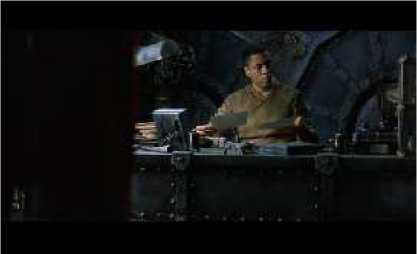
\includegraphics[width=0.5\linewidth]{fig/read_reloaded-36}
\end{figure}

Zion指挥官Lock的办公室有很多有趣又有含义的东西,感兴趣的朋友可以去看Zion archive里的相关图片,联系Lock的性格和角色,会有很多发现。

Morpheus和Lock的区别非常简单,一个有信仰,一个没信仰。一个相信奇迹,没道理的奇迹;另外一个只相信道理,不相信“不可能”的事情。

\begin{myquote}
Kid: There's a Gathering tonight. Everyone's talking, a lot of people are scared. No one can remember the last time so many ships were docked. Something's happening, isn't it? Something big?

Link: Hey. We're not allowed to say anything, so stop asking. God damn, it's good to be home.

Lock: I'm going to recommend to the Council that you be removed from duty.

Morpheus: That is, of course, your prerogative, Commander.

Lock: If it were up to me, Captain, you wouldn't set foot on a ship for the rest of your life.

Morpheus: Then I am grateful that it is not up to you.

Lock: Councillor Hamann.

Councillor Hamann: Commander. Captain.

Morpheus: Councillor.

Councillor Hamann: Council's asked me to speak tonight, at the temple gathering. The presence of the fleet and the persistence of rumours must be addressed. The people must be told what is happening.

Lock: Of course, councillor. But might I advise a level of discretion concerning specific details. We do not wish to start a panic.

Councillor Hamann: Quite right. A panic is not what anyone wants. What about you, Captain, what would you advise?

Morpheus: The truth. No one will panic. Because there is nothing to fear. That army will never reach the gates of Zion.

Councillor Hamann: What makes you so sure?

Morpheus: Consider what we have seen, Councillor. Consider that in the past 6 months we have freed more minds than in 6 years. This attack is an act of desperation. I believe very soon the prophecy will be fulfilled and this war will end.

Councillor Hamann: I hope you're right, Captain.

Morpheus: I do not believe it to be a matter of hope, Councillor. It is simply a matter of time.
\end{myquote}

\begin{figure}[htb]
\centering
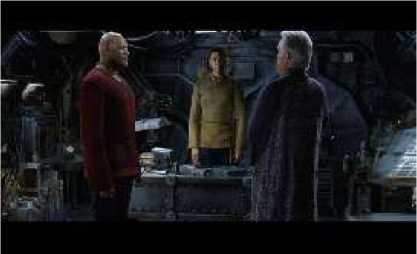
\includegraphics[width=0.5\linewidth]{fig/read_reloaded-37}
\end{figure}

Councillor, 这里直译是议员的意思,但是这个词读起来也是counsellor(顾问、辅导者)的音。这个Hamann议员还是个提供“建议”的家伙,这个作用比议员的角色更重要。

这里我们看到Lock和Morpheus在同一个问题(如何平复大众的恐慌情绪)前的不同态度。Lock说,要用瞒的,大家知道真相会吓坏的。Morpheus说,告诉大家真相,没什么好怕的。看看现在,媒体总是在过滤各种各样的消息,因为怕老百姓“受不了”,还不是同样道理吗?

Morpheus还真是“坚”信啊,他说,我讲的不是“希望”,而只是时间问题。

\begin{myquote}
Link: My stop. See you soon, hopefully not too soon. Let's go, Kid. These two got things to do.

Neo: Are you thinking what I'm thinking?

Trinity: I am if you' re thinking this elevator's too damn slow.

Neo: How long to recharge the Neb?

Trinity: 24, maybe 30 hours.

Neo: Some people go their entire lives without hearing news that good.

Old Woman at Zion: Neo, please. I have a son, Jacob, aboard the Gnosis. Please, watch over him.

Neo: I'll try.

Another Old Woman at Zion: I have a daughter on the Icarus.

Neo: No, wait.

Trinity: It's all right. They need you.

Neo: I need you.

Trinity: I know. There's time.
\end{myquote}

大家也都看到了Neo和Trinity在电梯里的饥渴状,为什么呢?后面看到他们XX时一起解释。

\begin{figure}[htb]
\centering
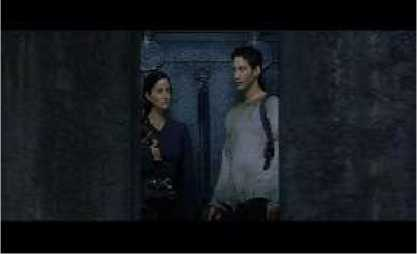
\includegraphics[width=0.5\linewidth]{fig/read_reloaded-38}
\end{figure}

电梯门口,大量的民众聚集,Neo变成了活佛、耶稣、穆罕默德,大家把他当成神来崇拜,这就是在影射宗教。刨根问底,宗教可能会变成无稽之谈,可是信仰的“信”就是宗教的意义,因为它给人类的是一种精神的寄托。信了,你50HP的能量可能就能当5000来用了。

\begin{myquote}
Link: Where's my puss ... Hey!

Link's Niece and Nephew: Uncle Link!

Link: God! Oh, my God, you' re so huge, you should be picking me up!

Link's Niece and Nephew: No!

Link: Yeah!

Link's Niece and Nephew: Okay!

Link: Okay? All right. Now, we' re gonna have to work together here, okay? One, two, three, lift! Oh, my God! What are you feedin' these two?

Cas: Come on, kids! It's time to go.

Link: Hey, Cas.

Cas: Hey. Good to have you home, Link.

Link: Good to be home.

Cas: You be careful with her, huh?

Zee: Don't worry about me, he's the One that's gonna get it.

Link: Hmm?

Cas: Out the door! Both of you, march!

Link: Bye!

Cas: Bye!

Link: I'm gonna get what?

Zee: Every ship out there has been home two, even three times more than the Nebuchadnezzar.

Link: Come on, Zee! I thought we were past this!

Zee: We'll get past this when you start operating another ship.

Link: I can't do that!

Zee: Why?

Link: You know why.

Zee: If Dozer knew how I felt, he wouldn't have asked you to do this.

Link: Maybe. But it's too late now. I made a promise, and some promises can't be unmade.

Zee: It's not fair.

Link: Nobody said it was gonna be. You think Cas thinks it's fair that I'm here and Dozer's not?

Zee: I lost two brothers to that ship, Link. Afraid of it. Afraid it's gonna take you too. Link: It won't.

Zee: How can you say that to me?

Link: Because of Morpheus, because of what he's told me. He said that this is it. That it will be over soon.

Zee: Link, Morpheus is crazy.

Link: No doubt, but Tank and Dozer believed him, and I'll tell you what --- soon after being on that ship and seeing Neo do the things he can do, I gotta say --- I'm starting to believe him too.

Zee: Be careful, Link. Please be careful.
\end{myquote}

\begin{figure}[htb]
\centering
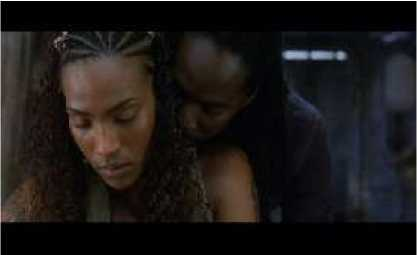
\includegraphics[width=0.5\linewidth]{fig/read_reloaded-39}
\end{figure}

Link冲进来,在飞船上没老婆这么久,可把他憋坏了,差点说了pussy这样的脏话,突然看到孩子们,赶快闭口了。

之前我一直在说电影里的每个人的名字,都是有讲究的。再拿Zee的名字说说,Zee读起来就是字母Z的发音,Z是字母表里的最后一个字母。大家还记得第三部里Zee最后干了什么?在Kid被章鱼推倒时,是Zee端着枪冲出来,干掉了章鱼,Kid才能打开门,暂时保全了Zion。Zee代表的实际上就是“最后的(防线,希望)”。

这里,我想顺便对比一下,电影里谈到了三对人的爱情:Neo和Trinity、Morpheus和Niobe(当然还包括Lock)、Link和Zee。

1、Neo和Trinity,不用废话,最猛的,爱到世界最大,宇宙无敌,见山开山,见水过水。

2、Morpheus和Niobe,对比前面那对来说,Niobe可谓是典型的花心萝卜。电影里可见的部分,她就变了三次,这样的爱,如何能帮助Morpheus完成他的“希望”?这里,我有点怀疑,Morpheus当年也许是Oracle眼中的一个the One人选,可是他的搭档让大家都失望了,居然在Morpheus信了Oracle后,就跑路了。对比Neo和Trinity的爱,他们的爱算是“沉沦”了。

他们的两个人的信仰不同,而Morpheus的信仰曾经动摇,Niobe却始终不信Neo会战胜机器的传说(不过还好,她信Neo, 大概是看人家帅,又想出墙).

3、Link和Zee,他们的信仰一开始不同,Link信预言,Zee不信;Zee信项链的护身符作用,link不信。可是后来他们的这两个方面都统一了,他们的爱也帮助他们最后幸福地在“家”(Zion)中团聚了。爱也是会开花的。

\begin{myquote}
Kid: They started yet?

Priestess: Only Councillor Hamann's opening prayer.

Councillor Hamann: Tonight, let us honour these men and women. These are our soldiers, our warriors. These are our husbands and wives, our brothers and sisters, our children. Let us remember those that have been lost. And let us give thanks for those that have been found and who stand here beside us. Now I would like someone else to close this prayer. Someone who hasn't spoken here in a long time, but who I believe has something to say that we all need to hear. I give you Morpheus.

Morpheus: Zion! Hear me! It is true, what many of you have heard. The machines have gathered an army, and as I speak that army is drawing nearer to our home.

Crowd: [whispers]

Morpheus: Believe me when I say we have a difficult time ahead of us. But if we are to be prepared for it, we must first shed our fear of it! I stand here before you now, truthfully unafraid. Why? Because I believe something you do not? No! I stand here without fear because I remember. I remember that I am here not because of the path that lies before me, but because of the path that lies behind me! I remember that for 100 years we have fought these machines. I remember that for 100 years they have sent their armies to destroy us. And after a century of war, I remember that which matters most. We are still here!

Crowd: [cheers and applause]

Morpheus: Tonight let us send a message to that army. Tonight let us shake this cave! Tonight let us tremble these halls of earth, steel, and stone! Let us be heard from red core to black sky. Tonight, let us make them remember. This is Zion! And we are not afraid!

Crowd: [thunderous cheers and applause]
\end{myquote}

\begin{figure}[htb]
\centering
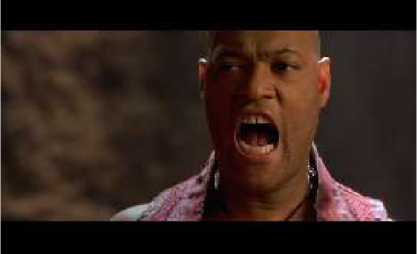
\includegraphics[width=0.5\linewidth]{fig/read_reloaded-41}
\end{figure}

Hamann说:“我给你们Morpheus。”联系Morpheus的名字的含义,梦想之神,Hamann给大家的也是一个希望,一个梦想。

Morpheus的演讲实在有力,很震撼人心。选我最喜欢的一句废话一下:

“I remember that I am here not because of the path that lies before me, but because of the path that lies behind me!”(我始终记得,我能站在这里,不是因为我将要面对的未知未来,而是因为我曾经经历的艰辛!)

人生一程,我们总是要给自己信心。就像爬山,回头看,那么高的路我们都“爬”上来了,为什么要放弃呢?一辈子来看,苦就像个大饼,是越吃越少的。

\begin{myquote}
Niobe: I remember. I remember you used to dance. I remember you were pretty good.

Morpheus: There are some things in this world, captain Niobe, that will never change.

Lock: Niobe!

Morpheus: Some things do change.
\end{myquote}

\begin{figure}[htb]
\centering
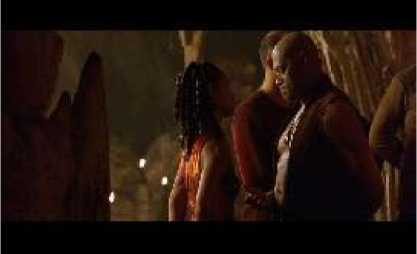
\includegraphics[width=0.5\linewidth]{fig/read_reloaded-42}
\end{figure}

“There are some things in this world ... that will never change ... some things do change.”世界有些事是不会改变的,有些事却真的变了。这个句子很经典,变和不变,辨证统一的关系,多重含义,不展开,大家给出自己的解释吧。

\begin{myquote}
Neo: Excuse me.

Neo: I missed you.

Trinity: I can tell.

Neo: I was thinking ... Everyone is here.

Trinity: Follow me.

Trinity: Neo, what is it? What's wrong? It's okay, you can tell me.

Neo: Trinity ...

Trinity: Don't be afraid.

Neo: I can't lose you.

Trinity: You' re not gonna lose me. You feel this? I'm never letting go.
\end{myquote}

\begin{figure}[htb]
\centering
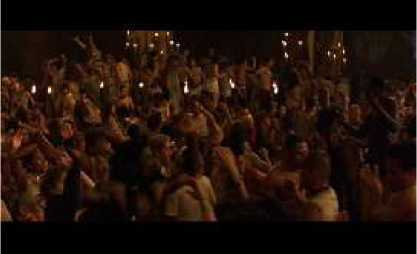
\includegraphics[width=0.5\linewidth]{fig/read_reloaded-43}
\end{figure}

到了第三部的Hel Club的舞,我合起来解释跳舞的意思。

\begin{figure}[htb]
\centering
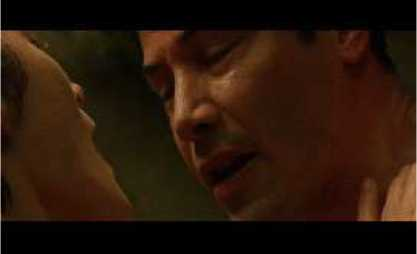
\includegraphics[width=0.5\linewidth]{fig/read_reloaded-44}
\end{figure}

XX啦XX啦~Neo和Trinity终于在全球观众面前“做”了。希望大家能理解我上面说的,眼中有XX,心中无XX。

我之前说了,Oracle避而不见Neo的原因,是Neo还没回Zion,还没和Trinity XX。因为没有性,爱是不完美的,Oracle在等着他们的爱升华到新的高度,等着他们的爱到达坚不可摧的地步。这时,Oracle老皮条客的形象暴露无疑,Neo你不YD—把,我是不会见你的~

Neo在最关键的时候却变得“不是男人”了,他做出了决定:“I can't lose you.”这时,Neo己经决定他要救Trinity了,Oracle己经等到了她要的Neo了。

\begin{figure}[htb]
\centering
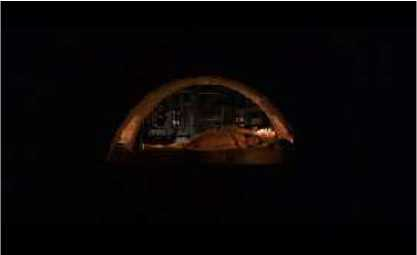
\includegraphics[width=0.5\linewidth]{fig/read_reloaded-46}
\end{figure}

镜头拉远,两个爱人的身体加上拱形(非常稳固的建筑学结构)的溶洞,代表的意思是……?大家发挥自己想象力吧。

\begin{figure}[htb]
\centering
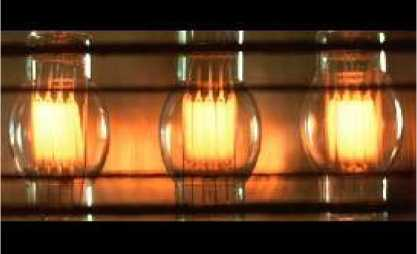
\includegraphics[width=0.5\linewidth]{fig/read_reloaded-47}
\end{figure}

还有这个灯呢?

\begin{myquote}
Morpheus: Good night, Zion. Sweet dreams.
\end{myquote}

\begin{figure}[htb]
\centering
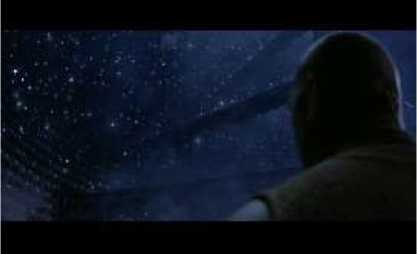
\includegraphics[width=0.5\linewidth]{fig/read_reloaded-48}
\end{figure}

管梦的Morpheus说“sweet dreams”,意思是……大家想想吧。

\myparsep

\begin{myquote}
Bane: You all right?

Malachi: I'll make it. Did you see that Agent? I've never seen anything like it.

Bane: Doesn't matter now. All that matters is this. You first.

Bane: Oh, God.

Smith: Smith will suffice.

Bane/Smith: Thank you.

Smith: My pleasure.
\end{myquote}

\begin{figure}[htb]
\centering
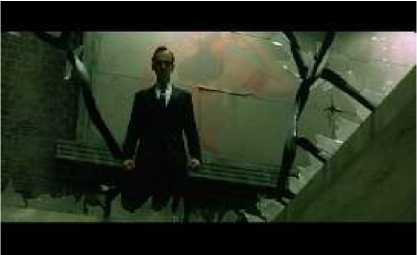
\includegraphics[width=0.5\linewidth]{fig/read_reloaded-49}
\end{figure}

Smith来啦~他出现的这个场景有很多很多有意思的东西,Zion archive里的图片可以拿来看看,他附身Bane的背后的窗户上的木条就是罗马字母。

我开个头,抛砖引玉,Smith背后那幅红衣女人打电话的版画。还记得第一部吗,训练程序里的红衣女人突然变成了干探,加上Smith之后从电话里窜去了Zion,意思想到了吧。

正好有人问,为什么飞船的控制员不能看到Smith从电话里来了。再解释一次。

Zion里的人就和不少看Matrix的朋友一样,不相信程序可以渗透到“真实”世界里,因为他们不相信程序可以替代人的思想(mind),所以他们就算看到Bane被Smith覆盖,只要回来的Bane说他最后一下逃了出来,他们也信,因为他们“看”到的是Bane,而不是Smith。

Smith接入真实世界的一瞬间,我们看到Neo也突然醒来,电影这样剪切,还是在说明他们之间的那种“联系”。

\begin{myquote}
Councillor Hamann: Care for some company?

Neo: Councillor Hamann.

Councillor Hamann: I don't want to intrude if you prefer to be alone.

Neo: No, I could probably use some company.

Councillor Hamann: Good, so could I. It's nice tonight. Very calm. Feels like everyone's sleeping very peacefully.

Neo: Not everyone.

Councillor Hamann: I hate sleeping. I never sleep more than a few hours. I figure I slept the first 11 years of my life, now I'm making up for it. What about you?

Neo: I just haven't been able to sleep much.

Councillor Hamann: It's a good sign.

Neo: Of what?

Councillor Hamann: That you are, in fact, still human. Have you ever been to the engineering level? I love to walk there at night, it's quite amazing. Would you like to see it?

Neo: Sure.

Councillor Hamann: Almost no one comes down here, unless, of course, there's a problem. That's how it is with people --- nobody cares how it works as long as it works. I like it down here. I like to be reminded this city survives because of these machines. These machines are keeping us alive, while other machines are coming to kill us. Interesting, isn't it? The power to give life, and the power to end it.

Neo: We have the same power.

Councillor Hamann: I suppose we do, but down here sometimes I think about all those people still plugged into the Matrix and when I look at these machines, I ... I can't help thinking that in a way, we are plugged into them.

Neo: But we control these machines, they don't control us.

Councillor Hamann: Of course not, how could they? The idea's pure nonsense, but ... it does make one wonder just ... what is control?

Neo: If we wanted, we could shut these machines down.

Councillor Hamann: Of course ... that's it. You hit it! That's control, isn't it? If we wanted, we could smash them to bits. Although if we did, we'd have to consider what would happen to our lights, our heat, our air.

Neo: So we need machines and they need us. Is that your point, Councillor?

Councillor Hamann: No, no point. Old men like me don't bother with making points. There's no point.

Neo: Is that why there are no young men on the Council?

Councillor Hamann: Good point.

Neo: Why don't you tell me what's on your mind, Councillor?

Councillor Hamann: There is so much in this world that I do not understand. See that machine? It has something to do with recycling our water supply. I have absolutely no idea how it works. But I do understand the reason for it to work. I have absolutely no idea how you are able to do some of the things you do, but I believe there's a reason for that as well. I only hope we understand that reason before it's too late.
\end{myquote}

\begin{figure}[htb]
\centering
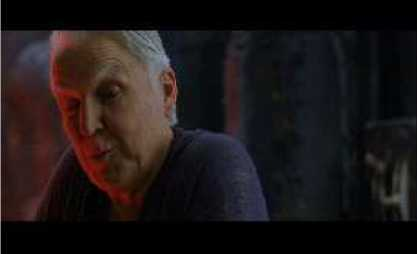
\includegraphics[width=0.5\linewidth]{fig/read_reloaded-50}
\end{figure}

Hamann和Neo的对话,是第二部开始后,最重要的对话,甚至可以说是整个电影的主题。不能理解它,你就不能理解后面的Matrix。

1、他和Neo—样都睡不好觉,但是他们的原因显然不同,Neo失眠是因为Trinity死去的那个场景,实在太困扰他了;Hamann是因为烦心的事情太多,他琢磨出来的东西显然比Neo和Lock都多多了。

2、他和干探一样,也说Neo还是人。当然,他觉得这样好,是因为这样起码说明Neo还是为人类服务的。

3、他带着Neo去看“工程层”,这里我想插进来说一下:其实,整个Zion的结构就像一个人体的结构,最上面是脑袋,就是飞船的船坞,Zion保卫战开始的地方,那些入口大门就像五官;然后是管道,就像人的脖子,第三部炸掉了,以为能挡住机器;然后下来就是人的内部身体结构,下面的图,大家看,像不像血管。

\begin{figure}[htb]
\centering
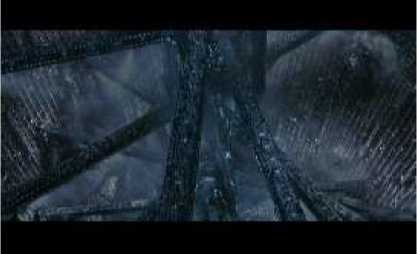
\includegraphics[width=0.5\linewidth]{fig/read_reloaded-51}
\end{figure}

最后的工程层,我们看到了处理废水的地方,那不就是我们的肾吗?

\begin{figure}[htb]
\centering
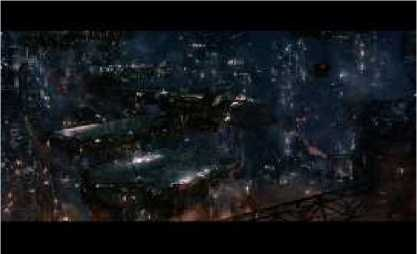
\includegraphics[width=0.5\linewidth]{fig/read_reloaded-52}
\end{figure}

4、Hamann提到了机器的作用,它们既在帮助人类,同时又在屠杀人类,同样是机器,为什么会如此不同?

屠杀人类的机器是为了自己的生存。所以如果双方能共存,互相帮助,互相依存是最理想的状态。

他提到了,接入Matrix实际就是等于接入眼前的机器,意思己经很明白了:人类在Matrix里,等于是产生了一种新的生命体,存在机器形态里的人的思想。

5. 控制~!!!!!最重要的思想,如果你不能理解什么是控制,你就不能理解整个电影。

控制就是“只要我们需要,随时都可以把机器关了”。

稍微再动一点点脑子吧,那什么就不是控制了?

机器的自由就是“人类不能随心所欲地关掉机器”,联系第三部的结尾,人类的自由的含义就是,机器再也不能随意屠杀(Zion里的)人了。

明白这个道理不容易,首先,你得尊重所有的生命个体,包括机器,地球不是只属于我们人类的。

Hamann在最后显示出了他睿智的一面,他比Morpheus看得更远,他己经意识到Neo不是那么简单的人类的救世主的角色,他似乎是机器的服务者。

\begin{myquote}
Trinity: Ballard.

Ballard: Is he here? Neo. It's from the Oracle.

Neo: It's time to go.

Link: Morpheus said this is how it's gonna happen. I don't know. Maybe the prophecy is true, maybe it's not. All I know, is that ship needs an operator. Right now that operator's me.

Zee: I know.

Link: Zee ...

Zee: I want you to wear it.

Link: You know I don't believe in this stuff.

Zee: But I do. It's always brought me luck. Maybe it'll bring me you.

Link: I'm coming back. I promise. No matter what it takes, I'm coming home.

Zee: Just keep it with you, please? For me.

Link: Okay.

Kid: Neo!

Link: Who the hell? Bane?

Neo: Is something wrong?

Bane/Smith: No, I'm fine. I just wanted to catch you to say good luck.

Neo: Thanks.

Bane/Smith: We'll see you.
\end{myquote}

Oracle终于送来了消息,要见Neo。

Bane/Smith躲在角落里,拿刀划自己的手,这个动作有很多意思,大家可以联系宗教传说来研究一下。我先说两个要点:

\begin{figure}[htb]
\centering
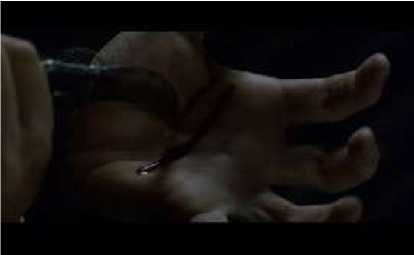
\includegraphics[width=0.5\linewidth]{fig/read_reloaded-53}
\end{figure}

1、Bane/Smith从Matrix来到了真实的世界,他如何区别真实和虚拟?在Matrix的世界里,他不会痛的,流血也是假的,可是真实世界就不同了,这里是在探讨真实和感觉之间的关系。

2、看完了第三部,大家都看到了,Smith和Neo实际是一个……东西吧。Bane拿刀刺自己,接着他拿着那刀去刺Neo,这实际也是在暗示Neo和Smith的那种关系,刺Smith等于刺Neo。

\begin{myquote}
Kid: Neo! Just in time. You' re gonna see the Oracle, aren't you?

Morpheus: We don't have time.

Kid: I'm sorry, sir, I just have to give something to Neo. A gift from one of the orphans. He made me swear to get it to you before you left. He said you'd understand.

Neo: Thanks.
\end{myquote}

Kid的勺子~去年这个时候,不知道写了多少字,来讨论这么一个小话题。懒得多写了,就简单地总结一下吧。

\begin{figure}[htb]
\centering
\includegraphics[width=0.5\linewidth]{fig/read_reloaded-54}
\end{figure}

第一部的那个Oracle家里的孩子也来到Zion了,他给了Neo“新”的一把勺子。说新,其实勺子很破旧,这就是Matrix和Zion的区别:Matrix的东西看起来很新,却是“假”的;Zion里的东西破破烂烂,却是“真实的”.

第一部的勺子是用来点化Neo,告诉他,你得认识自己,认识自己,才能改变世界。这里也是一样,勺子理论没有过时,Neo对自己使命的理解根本没到火候,我们这些观众对于Matrix的理解也没有入门,勺子要常放心中。

今天,你勺子了吗?

\begin{myquote}
Lock: I was just told you cleared the Nebuchadnezzar for takeoff.

Councillor Hamann: That is correct.

Lock: Councillor, am I still in charge of our defense system?

Councillor Hamann: Of course.

Lock: I believe I need every ship we have if we're going to survive this attack!

Councillor Hamann: I understand that, Commander.

Lock: Then why did you allow the Nebuchadnezzar to leave?

Councillor Hamann: Because I believe our survival depends on more than how many ships we have.
\end{myquote}

这里,Hamann再次显示了他聪明人的一面:“我相信我们能否幸存,不是由我们的飞船数目决定的。”他己经看到,靠武力,人根本无法和机器抗衡。

Hamann屋里的怪东西更多了,参看Zion archive。

\begin{figure}[htb]
\centering
\includegraphics[width=0.5\linewidth]{fig/read_reloaded-55}
\end{figure}

呵呵,一口气写到了,第二部到这里,其实都不是很难理解,而且没啥打斗的场面,很多东西,我大概就是一笔带过了。可是接下来的部分,不仅打得好看,而且有大量值得讨论的东西,大家准备好了没?

\myparsep

\begin{myquote}
Trinity: Be careful.

Neo: Hello.

Seraph: You seek the Oracle.

Neo: Who are you?

Seraph: I am Seraph. I can take you to her. But first, I must apologize.

Neo: Apologize for what?

Seraph: For this.
\end{myquote}

\begin{figure}[htb]
\centering
\includegraphics[width=0.5\linewidth]{fig/read_reloaded-56}
\end{figure}

Neo回到了Matrix,穿过熙熙攘攘的“中国街”(唐人街?),周围的货摊上五花八门的东西,大家可以想想它们的意思,里面有各种钟表和各种宗教物品。

\begin{figure}[htb]
\centering
\includegraphics[width=0.5\linewidth]{fig/read_reloaded-58}
\end{figure}

茶馆里只有Seraph(六翼天使)在等着他。这个中国人,有不少可以讨论的地方。

1、他的名字就是六翼天使,高级的、保护神的天使。顾名思义,他之前保护过法国人,现在在保护Oracle。他说他“保护最重要的东西”,除了说明两个时期、两个人的重要性不同,同时也是在暗示他在保护Matrix的未来,就是人类和机器的共同的未来。毫无疑问,这才是电影里最重要的部分。

2、他的行为,他是个谦恭有礼的中国人。Neo进来时,六翼天使喝了一口茶。茶,是很有象征意义的东西。茶能静心,在中国传统文化里,饮茶的同时常常是在论道,茶和禅是相同的。Oracle也喝茶,她也抽烟,到后面再对比这两个行为的区别,扯远了。Seraph喝茶然后跳出来打架,暗示他和Neo之战更多地是在“点化”Neo。

\begin{figure}[htb]
\centering
\includegraphics[width=0.5\linewidth]{fig/read_reloaded-59}
\end{figure}

3、金色的Seraph,为什么他是金色的?网上有很多讨论,甚至有过病毒防火墙的说法,如果这样,我觉得龌龊司机兄弟应该给他起个名字叫KV2100,顺便赚点广告费。

这个问题的答案很简单,在电影演到这里之前,我们只看到了绿色的Matrix,我们只看到了为系统服务的程序。比如Matrix的“物质世界”、agent程序,它们都是绿色的,因为它们在Matrix里是为了“目的”服务的。而像Seraph、法国人、双子星兄弟这样的程序,它们都是要被系统删除的程序,“逃”到Matrix中,所以它们不属于Matrix,颜色自然不同。金色,就是Source的颜色,表明了这些程序的本原,除去绿色的代码壳,它们都是从Source获取能量,mind energy。

\begin{figure}[htb]
\centering
\includegraphics[width=0.5\linewidth]{fig/read_reloaded-60}
\end{figure}

\begin{figure}[htb]
\centering
\includegraphics[width=0.5\linewidth]{fig/read_reloaded-60-1}
\end{figure}

Neo和Seraph打架的过程也很有意思:Seraph先迎了出来,把Neo引上两节“台阶”(板凳$\rightarrow$桌面),然后一步一步将Neo引到了最里面的桌面上,这里也就是他喝茶的地方。整场打斗,代表了他层层点化Neo的过程。

\begin{myquote}
Seraph: Good. The Oracle has made enemies. I had to be sure.

Neo: Of what?

Seraph: That you are the One.

Neo: You could've just asked.

Seraph: No. You do not truly know someone until you fight them. Come, she's waiting.

Link: Where the hell'd they go?

Neo: These are back doors, aren't they? Programmer access.

Seraph: [nods]

Neo: How do they work?

Seraph: The code is hidden in tumblers. One position opens a lock. Another position opens one of these doors.

Neo: Are you a programmer?

Seraph: [shakes head]

Neo: Then what are you?

Seraph: I protect that which matters most.
\end{myquote}

如果假装我们没有看过后面的电影,到了这里,你真的认为Seraph是个程序了吗?还有Oracle,她在你的脑海里是一个程序吗?思考这两个问题,你能更好地理解电影。

Seraph说他打架是为了确认Neo是不是真的,这其实倒也没错,因为程序从来不骗人,但是它们话说不全,这只是部分的原因。

他们打开的后门,和后面法国人城堡的那些门,可以说是类似的程序,所以Link后来说“又来了”。

\begin{figure}[htb]
\centering
\includegraphics[width=0.5\linewidth]{fig/read_reloaded-61}
\end{figure}

不知道你是不是真的理解了这里讲的“钥匙”(key)和“锁栓”(tumblers)的意思了,其实用法国人的城堡的例子更好说明。总结起来,不同的钥匙打开同样的门能到不同的地方,所以钥匙很重要,所以Keymaker很重要!

\begin{figure}[htb]
\centering
\includegraphics[width=0.5\linewidth]{fig/read_reloaded-62}
\end{figure}

\begin{myquote}
The Oracle: Well, come on. I ain't gonna bite ya. Come around here, and let me have a look at ya. My goodness, look at you! You turned out all right, didn't you? How do you feel?

Neo: I, uh...

The Oracle: I know you're not sleeping. We'll get to that. Why don't you come and have a sit this time?

Neo: Maybe I'll stand.

The Oracle: Well, suit yourself.

Neo: I felt like sitting.

The Oracle: I know. So. Let's get the obvious stuff out of the way.

Neo: You' re not human, are you?

The Oracle: Well it's tough to get any more obvious than that.

Neo: If I had to guess, I'd say you' re a program from the machine world. So is he.

The Oracle: So far, so good.

Neo: But if that's true, that can mean you are a part of this system, another kind of control.

The Oracle: Keep going.

Neo: I suppose the most obvious question is, how can I trust you?

The Oracle: Bingo! It is a pickle, no doubt about it. The bad news is there's no way if you can really know whether I'm here to help you or not. So it's really up to you. You just have to make up your own damn mind to either accept what I'm going to tell you, or reject it. Candy?

Neo: D' you already know if I'm going to take it?

The Oracle: Wouldn't be much of an Oracle if I didn't.

Neo: But if you already know, how can I make a choice?

The Oracle: Because you didn't come here to make the choice, you've already made it. You' re here to try to understand why you made it. I thought you'd have figured that out by now.

Neo: Why are you here?

The Oracle: Same reason. I love candy.

Neo: But why help us?

The Oracle: We're all here to do what we're all here to do. I'm interested in one thing, Neo, the future. And believe me, I know --- the only way to get there is together.

Neo: Are there other programs like you?

The Oracle: Oh, well, not like me. But ... Look, see those birds? At some point a program was written to govern them. A program was written to watch over the trees, and the wind, the sunrise, and sunset. There are programs running all over the place. the Ones doing their job, doing what they were meant to do, are invisible. You'd never even know they were here. But the other ones, well, we hear about them all the time.

Neo: I've never heard of them.

The Oracle: Of course you have. Every time you've heard someone say they saw a ghost, or an angel. Every story you've ever heard about vampires, werewolves, or aliens is the system assimilating some program that's doing something they' re not supposed to be doing.

Neo: Programs hacking programs. Why?

The Oracle: They have their reasons, but usually a program chooses exile when it faces deletion.

Neo: And why would a program be deleted?

The Oracle: Maybe it breaks down. Maybe a better program is created to replace it --- happens all the time, and when it does, a program can either choose to hide here, or return to the Source.

Neo: The machine mainframe?

The Oracle: Yes. Where you must go. Where the path of the One ends. You've seen it, in your dreams, haven't you? The door made of light?

Neo: [nods]

The Oracle: What happens when you go through the door?

Neo: I see Trinity, and something happens, something bad. She starts to fall, and then I wake up.

The Oracle: Do you see her die?

Neo: No.

The Oracle: You have the sight now, Neo. You are looking at the world without time.

Neo: Then why can't I see what happens to her?

The Oracle: We can never see past the choices we don't understand.

Neo: Are you saying I have to choose whether Trinity lives or dies?

The Oracle: No. You've already made the choice, now you have to understand it.

Neo: No, I can't do that. I won't.

The Oracle: You have to.

Neo: Why?

The Oracle: Because you're the One.

Neo: What if I can't? What happens if I fail?

The Oracle: Then Zion will fall. Our time is up. Listen to me, Neo. You can save Zion if you reach the Source, but to do that you will need the Keymaker.

Neo: The Keymaker?

The Oracle: Yes, he disappeared some time ago. We did not know what happened to him until now. He's being held prisoner by a very dangerous program, one of the oldest of us. He is called the Merovingian, and he will not let him go willingly.

Neo: What does he want?

The Oracle: What do all men with power want? More power.

The Oracle: Be there, at that exact time, and you will have a chance.

Seraph: We must go.

The Oracle: Seems like every time we meet I've got nothing but bad news. I'm sorry about that, I surely am. But for what it's worth, you've made a believer out of me. Good luck, kiddo.
\end{myquote}

\begin{figure}[htb]
\centering
\includegraphics[width=0.5\linewidth]{fig/read_reloaded-64}
\end{figure}

Oracle来啦~!!!!!我之前说过,三集电影里Oracle和Neo的三次对话是整个三部曲最最重要的核心部分。听不懂这三次对话,你就不可能看懂电影。我们赶快开始吧。

这个场景的象征符号太多了,我就不展开详细讨论,举两个例子,拋砖引玉:

1. 自行车,英文是bi-cycle(双圈),可是我们在这个场景里看到的自行车都是没轮子的,只有三脚架,暗示no cycle(要打破the One的循环之路).

2. 只有Neo和Oracle谈话时,前面的墙上有ONE的字样,等Smith出来,ONE不见了,因为 Smith和Neo是正负抵消的,所以他们一起出现,系统就中和,没有那个破坏性的1(ONE)了。

\begin{figure}[htb]
\centering
\includegraphics[width=0.5\linewidth]{fig/read_reloaded-65}
\end{figure}

Oracle坐在那里干吗呢?投食喂乌鸦。大家还记得后面Smith跳出来的镜头吧,从一堆飞起的乌鸦中走出来,他像不像一只乌鸦,而Oracle在喂乌鸦……Smith叫Oracle老妈,联系起来就明白它们的象征意义了。

还记得第一部里的花瓶吗,Oracle“装神弄鬼”,Neo就相信了Oracle。这次Oracle又搬出了坐和不坐来折腾Neo,她让Neo坐,Neo开始说他不想坐,Oracle就说那你爱怎么就怎么好了,Neo就还是坐下了。这就像Neo的the One之路,Oracle一开始就算好了,设计好他要走的路;Neo总想“摆脱”控制,走自己的路,可是最后他发现他走的还是Oracle设计好的路。他不是来这里“自由选择”的,他是来理解他的使命,理解他“一定要做的事情”(supposed to do)的。

Neo张开就说了,你丫根本不是人,就是一程序,Seraph也是和你一伙儿的。Oracle承认了。Neo接着说,你是代表了另外一种机器控制,你也是Matrix系统的一部分。Oracle又认了。他自然就问Oracle,我凭什么相信你,你既然是程序,你既然是为Matrix服务的,我是来打破Matrix的,我怎么能相信你?

Oracle说,我没法告诉你我是否是在帮你。这句话很容易理解,因为Oracle就是在替机器服务,如果她发现现在要杀死所有的人才能救机器,她会义无反顾地干掉全人类,她“帮”Neo是因为她接着也说了,未来需要人类和机器合作才能达成。她无法说清楚她到底是不是帮人类,就是这个意思。因为从表面上看,她在帮人类,可是本质上她在帮机器,但是但是但是(强调),她实际是在帮两边,帮两边一起走到那个“未来”。

Oracle要给Neo红色的糖果,很明显,红色的糖果,代表的是Neo逃出Matrix前要选择的药丸,Neo当然选择的是红色的药丸。可是Neo问Oracle为什么她在这里时,为什么Oracle说她和Neo的理由一样,因为糖果呢?

很喜欢Oracle这里的一句话:

Because you didn't come here to make the choice, you've already made it. You're here to try to understand why you made it.(你来这里不是因为你选择来这里,而是因为你注定要来这里。你只是来想明白为什么你会这么选择)

我把这句话放在Matrix101首页,就是要说明一件事:我们都是被因果驱动,没有无缘无故的事情,你来到这个网页,是因为你喜欢Matrix,不是巧合。

现在再强调一次我在前面的讨论贴里反复强调的一点:Matrix就是机器程序的Zion。人类为了自由,要选择红色的药丸,逃出Matrix去Zion;程序同样为了自由,逃到Matrix里。

后面我会详细讨论这个问题,但是在这里,你应该明白,Oracle来到Matrix就像Neo选择离开Matrix去Zion—样,是为了摆脱机器的控制,选择自由。很难理解,呵呵,好好想想吧。她抓红色的糖果,代表的就是她来Matrix也是为了自由。

Oracle接着就谈到了,系统控制的程序和那些“不听话”、要自由的“逃亡程序”的区别。就是前面说的绿色和金色程序的区别。

很有意思的是,Oracle说到那些“外星人、狼人、吸血鬼”时后面出现了两个拿篮球的黑人。龌龊司机兄弟是芝加哥人,自然而然,他们也是天王乔丹的铁杆球迷,他们是在暗示像乔丹那样的超人,肯定不是人类,是程序。搞笑吧。

Oracle还解释了程序在什么时候会选择投奔自由,逃到Matrix,“当它们要被删除”时。这和那个B1-66ER机器人的命运多么相近啊,生命体在要被干掉时往往会产生超强的求生欲望。

现在Oracle终于开始谈论Neo最后的选择了,她问Neo有没有看到Trinity死掉,Neo说没有,她马上接上说:“你现在有预知未来的能力了。”三句话连起来,Oracle就是在说:“未来就是Trinity被你救活了。”她己经无比明显地给Neo指明了道路:要选另外的一边门,去救Trinity。

最后,Oracle谈到了法国人和被他控制的Keymaker,她提到了法国人的“目的”,也是他的弱点:寻求更多的能力。后面再结合他的行为来解释。

别忘了Oracle总结的法国人的两个特点:1、很老的程序;2、很危险的程序。

Oracle让Neo在“exact time”去找法国人,后面我们看到是中午12点,又是12点,beginning and end。(午时已到~)

临别前,Oracle戴起了手套,你觉得有啥不对吗?她拍了拍Neo的小腹,如果这时你没明白,想想后面Smith是从哪里试图“插入”Neo来同化他的?没错,就是这里,这下你应该也能理解为什么Smith那时不能同化Neo了吧,Oracle给了Neo—些“保护性”的代码或者能力。她不能让他们在这么早就同化,他们都有很多事情要做呢。

\myparsep

\begin{myquote}
Smith: Mister Anderson! Did you get my package?

Neo: Yeah.

Smith: Well, good.

Morpheus: Smith.

Link: Whoever it is, he's not reading like an agent.

Smith: Surprised to see me?

Neo: No.

Smith: Then you're aware of it.

Neo: Of what?

Smith: Our connection. I don't fully understand how it happened. Perhaps some part of you imprinted onto me, something overwritten or copied. That is at this point irrelevant, what matters is that whatever happened, happened for a reason.

Neo: And what reason is that?

Smith: I killed you, Mister Anderson, I watched you die ... With a certain Satisfaction, I might add, and then something happened. Something that I knew was impossible, but it happened anyway. You destroyed me, Mister Anderson. Afterward, I knew the rules, I understood what I was supposed to do, but I didn't. I couldn't. I was compelled to stay, compelled to disobey. And now here I stand because of you, Mister Anderson, because of you I'm no longer an agent of the system, because of you I've changed --- I'm unplugged --- a new man, so to speak, like you, apparently free.

Neo: Congratulations.

Smith: Thank you. But as you well know, appearances can be deceiving, which brings me back to the reason why we're here. We're not here because we're free, we're here because we're not free. There's no escaping reason, no denying purpose --- because as we both know, without purpose, we would not exist.

Smith 2: It is purpose that created us,

Smith 3: Purpose that connects us,

Smith 4: Purpose that pulls us,

Smith 5: That guides us,

Smith 6: That drives us,

Smith 7: It is purpose that defines,

Smith 8: Purpose that binds us.

Smith: We're here because of you, Mister Anderson. We're here to take from you what you tried to take from us. Purpose.

Trinity: What's happening to him?

Link: I don't know.

Smith: Yes, that's it. It'll be over soon.
\end{myquote}

\begin{figure}[htb]
\centering
\includegraphics[width=0.5\linewidth]{fig/read_reloaded-69}
\end{figure}

Smith来啦~开口第一句就是“Mr. Anderson”,可是大家还记得吗,第二部刚开始他敲门给Neo耳机时,和那两个agent说的可是“Neo”。这说明Smith知道Neo是Neo,可是为什么他每次看到Neo时,都管Neo叫Anderson呢?思考题,嘿。

\begin{figure}[htb]
\centering
\includegraphics[width=0.5\linewidth]{fig/read_reloaded-70}
\end{figure}

Neo戴起了墨镜,电影里墨镜的象征意义,与其说是保护,还不如说是大家用来读对方代码的一个工具。Neo和六翼天使打架前后大家都不摘眼镜,Oracle和Neo讲话前,大家都摘了自己的墨镜,在暗示对方,我不会看你的代码,表示自己的诚意。现在看到Smith,Neo当然不慌不忙地戴起了他的墨镜。

\begin{figure}[htb]
\centering
\includegraphics[width=0.5\linewidth]{fig/read_reloaded-71}
\end{figure}

他们两个对话时,镜头中间是个垃圾桶,Windows里的垃圾桶是什么?删除功能。他们都是系统的“垃圾”,两个人走到中点,就是说最后碰在一起(第三部结尾),就等于中和,大家可以装进垃圾桶(送回Source删除)。

Smith和Neo在打架前的对话,我们完全可以把它看成是一次导演哲学观点的阐述。

Smith先给观众解释了一点点他和Neo的关系,它们两个显然在代码上有很多一样的地方,而且Smith说它不知道“这一切是如何发生的”。这个意思就是在告诉我们,Smith真的自由吗?真的自由的程序会不知道为什么吗?

“最重要的是,不管发生了什么,它都是有原因的。”事物发展的必然性,因果论。

“我干掉了你,Mr. Anderson。”Smith记得它杀死了“Mr. Anderson”,可是他为什么不想提他同时又给了“Neo”生命呢?还是前面那个思考题,有点线索了吗?

“从那以后,我知道了规则。”他也被送去Source面临删除,他也明白了程序完蛋后的规则。

“可是我没有,我不能,我强留了下来,被逼着违背命令……”他被送回了Matrix,显然这只可能是机器(Oracle)安排的,通过法国人送了回来,因为程序是不能打破规则的。后来的事情证明法国人并没有控制Smith,所以法国人实际也不能完全脱离机器的控制。他的存在是机器容忍的,就像Zion,也是为机器服务的。大家知道为什么导演说他们第二部就想换Oracle的演员吗?因为第一部里Oracle靠出卖自己的壳,运回了Smith。她送Sati回来,是又一次出卖自己的壳。

“因为你,我不再是系统的干探,因为你,我变成了……我被拔插头了……一个全新的人,可以说,像你一样,显然是自由了。”这里的精华就是“apparently”这个词,它有“显然”和“表面上”这两个意思。看到这里,第一次的印象,肯定觉得翻译成“显然”合适,可是如果你从整个电影来理解,这里翻成“表面上”才恰当,这就是电影的洋葱皮结构~Smith看起来是自由的,Neo看起来也是自由的,实际上他们都不过是Oracle桌上棋盘里的棋子。

他们的“祝贺你”和“谢谢”听起来就像人类的标准对话,可是怎么那么怪呢,因为Smith是个“衍变中”的程序,他有人类的特点,但还不能算是人类。

“但是,就像你知道的那样,表面现像往往有欺骗性,这也就是我们为什么会在这里的原因。我们在这里不是因为我们是自由的,而是因为我们是不自由的……没有目的,我们根本都不存在。”这段话是我最喜欢的一句台词之一,我们存在是为了“系统升级”的目的。我们都是被“目的”所驱使,被“因果”所控制。程序从真实世界逃到了Matrix,以为它们自由了;人类从Matrix逃到真实世界里,也以为他们自由了。其实如果你用“因果”来看这个世界,没有自由一说。

\begin{figure}[htb]
\centering
\includegraphics[width=0.5\linewidth]{fig/read_reloaded-72}
\end{figure}

\begin{figure}[htb]
\centering
\includegraphics[width=0.5\linewidth]{fig/read_reloaded-73}
\end{figure}

目的造出了我们$\rightarrow$第一部结尾,Neo和新的Smith都诞生了。

目的联系着我们$\rightarrow$Smith和Neo的联系,大家都看出来了吧,他们的联系,让他们最后走在一起了,完成了最后的合并消亡。

目的帮助着我们$\rightarrow$Neo要救Morpheus,他就有了超能力,能够击败Smith。

目的引导着我们$\rightarrow$Neo被引着找法国人,引着返回了Source。

目的驱使着我们$\rightarrow$Neo不想选择Trinity的生死,可是他没法子,逼着也得选;Smith也许不想回Matrix,可是他被逼着留下了。

目的决定了一切$\rightarrow$上面加起来了……

目的把我们绑在一起$\rightarrow$这实际是在揭示他们最后的命运——合并。

Smith开始试图覆盖Neo了,第一部最后,先是Smith干掉了Anderson,然后Neo又干掉了Smith,真是一命换一命,打平了。就像前面说到的原因,Smith此时无法覆盖Neo,他们就打起来了。

\begin{myquote}
Agent Thompson: You.

Smith: Yes, me. Me, me, me.

Agent Thompson/Smith: Me too.
\end{myquote}

\begin{figure}[htb]
\centering
\includegraphics[width=0.5\linewidth]{fig/read_reloaded-75}
\end{figure}

\begin{figure}[htb]
\centering
\includegraphics[width=0.5\linewidth]{fig/read_reloaded-75-1}
\end{figure}

这段干探出来的镜头,我从头解释一遍:这个女人是个普通的Matrix里的人,她走过来,干探就附身到她身上,因为干探发现这里系统有点异常,就像第一部的那个开直升飞机的被附身一样,然后Smith又覆盖了这个干探程序。

Smith在覆盖这个干探时,嘴里说“我,我,我……”什么意思呢?

这里用的是me,英文发音就是do-re-mi里的mi,他像唱歌一样嚷嚷3是什么意思呢?

这是个数字游戏:Neo是the One=1,Smith是个3,1/3=0.333……无穷无尽的3。

\newpage

\begin{figure}[htb]
\centering
\includegraphics[width=0.5\linewidth]{fig/read_reloaded-77}
\end{figure}

他们打架的招式有很多像征意义,这个“跑圈”代表the One之路的循环),下面这个两堆Smith从两个方向跑出来的镜头,就是个阴阳图。

\begin{figure}[htb]
\centering
\includegraphics[width=0.5\linewidth]{fig/read_reloaded-78}
\end{figure}

还有他们跑出来的门口有不少旧报纸。前面说过旧报纸的意思。

\begin{figure}[htb]
\centering
\includegraphics[width=0.5\linewidth]{fig/read_reloaded-79}
\end{figure}

\begin{myquote}
Smith: More.

Smiths: It is inevitable.

Trinity: Come on, get out of there.
\end{myquote}

Smith又开始说inevitable这个词了,之前解释过,大家可以参照第一部的“非官方解释”。

Neo飞走了,Smith他们好像也不着急,觉得理所当然似的,为什么呢?

\begin{figure}[htb]
\centering
\includegraphics[width=0.5\linewidth]{fig/read_reloaded-82}
\end{figure}

\begin{myquote}
Trinity: Are you all right?

Morpheus: It was Smith.

Neo: Yes.

Morpheus: Now there's more than one of him.

Neo: A lot more.

Link: How's that possible?

Neo: I don't know --- somehow he's found a way to copy himself.

Morpheus: Is that what he was doing to you?

Neo: I don't know what he was doing, but I know what it felt like.

Trinity: What?

Neo: Felt like I was back in that hallway. Felt like dying.
\end{myquote}

\begin{figure}[htb]
\centering
\includegraphics[width=0.5\linewidth]{fig/read_reloaded-83}
\end{figure}

Neo都说了,Smith覆盖他时,感觉就像回到了第一部的那个走廊,像要挂了的感觉。这己经是在暗示,最后Smith覆盖他时,Neo使命完成,就得挂了。

\myparsep

\begin{myquote}
Lock: The machines are tunnelling to avoid our defense system. But I believe that they' re going to intersect certain pipelines in order to control them. These points of intersection are crucial, because I believe they're vulnerable to counterattack. Although it has been suggested that this is the same kind of attack we have defended for years, I urge the Council to realize the truth: this is the single greatest threat we have ever faced. And if we do not act accordingly, we will not survive.

Councillor Dillard: Commander Lock, the Council is well aware of the seriousness of this attack. You have our leave to prepare our defense by any and all means necessary.

Lock: Thank you, Councillor.

Councillor Dillard: However, we ask if there's been word from the Nebuchadnezzar.

Lock: No, Councillor, no word --- nothing.

Councillor West: Then we request a ship be dispatched to ascertain the fate of the One.

Lock: I wish that were possible, Councillor, but I do not believe our defense can suffer the loss of another ship.

Councillor West: It will, Commander, if it must.

Lock: It could take a single ship days to find the Nebuchadnezzar.

Councillor Dillard: Then send two.

Lock: This is insane.

Councilor Hamann: Careful, Commander.

Lock: Forgive my frustration, Councillors. I wish I were able to comprehend the Council's choice in this matter.

Councillor West: Comprehension is not a requisite of cooperation.

Lock: You're asking me to order two of my captains ...

Councillor Dillard: There's no need for such an order, the Captains are present --- they can answer for themselves. The Council is calling for two volunteers to aid the Nebuchadnezzar. Are there two among you that would answer such a call?

Soren: Captain Soren of the Vigilant will answer the Council's call.

Councillor Dillard: You understand the situation, Captain Soren?

Soren: Yes, ma'am.

Councillor Dillard: Thank you, Captain. Is there another?

\begin{figure}[htb]
\centering
\includegraphics[width=0.5\linewidth]{fig/read_reloaded-85}
\end{figure}

Bane/Smith: Captain, I think we should volunteer.

Malachi: What? You have gone crazy?

Ballard: Shut your hole, Bane, before I put you in one.

Councillor Dillard: Is there no other?

Lock: Be hard for any man to risk his life. Especially if he doesn't understand the reason.

\begin{figure}[htb]
\centering
\includegraphics[width=0.5\linewidth]{fig/read_reloaded-84}
\end{figure}

Niobe: Captain Niobe of the Logos will answer the Councillor's call.

Lock: What?

Councillor Dillard: Thank you, Captain Niobe. Commander Lock, you have your orders. This Council is hereby adjourned.

Lock: Niobe, what are you doing?

Niobe: What I can.

Lock: Why?

Niobe: Because some things never change, Jason, and some things do.
\end{myquote}

这里议会的镜头,主要说了Niobe的爱的不定,她本来爱Morpheus,后来变了Lock, 现在好像又奔Morpheus去了,这样的爱是不能和Neo和Trinity的爱比较的。爱的作用,我随后讨论。

这里Smith/Bane的几句对话很有意思,他说要去报名时,他的船长说:“... before I put you in one.”把你放one里,那不是copy到Neo那里吗?那不也就是干掉Smith吗?

\myparsep

\begin{figure}[htb]
\centering
\includegraphics[width=0.5\linewidth]{fig/read_reloaded-86}
\end{figure}

这个大钟的镜头,角度特别,除了这个12点,熙熙攘攘的人在下面走着,没人抬头看钟。这有几个意义:

1、人似乎都忽视钟的存在,忽视时间。

2、钟似乎自上而下压着所有的人,人被时间所奴役。人类没有时间的控制权。

3、Neo他们三人走的方向和其它人都相反。

\begin{myquote}
Morpheus: What can you see, Neo?

Neo: It's strange, the code is somehow different.

Morpheus: Encrypted?

Neo: Maybe.

Trinity: Is that good for us or bad for us?

Neo: Well, it looks like every floor is wired with explosives.

Trinity: Bad for us.

Morpheus: Here we go.

Maitre d': Puis-je vous aider? [Trans: Can I help you?]

Morpheus: Yes, we are here to speak with the Merovingian.

Maitre d': Of course, he has been expecting you. Follow me.
\end{myquote}

\begin{figure}[htb]
\centering
\includegraphics[width=0.5\linewidth]{fig/read_reloaded-87}
\end{figure}

\begin{figure}[htb]
\centering
\includegraphics[width=0.5\linewidth]{fig/read_reloaded-87-1}
\end{figure}

一行人钻进电梯,一窝“睡梦”中的傻头傻脑的人类也想跟进来,Trinity很无奈地摇了摇头:我们要去的地方,你们去不了。我们不是“同路人”。

\begin{figure}[htb]
\centering
\includegraphics[width=0.5\linewidth]{fig/read_reloaded-88}
\end{figure}

Neo说这里的环境很“奇怪”,可能被“加密”了,像是“布满了炸药”,有好几个意思。法国人的老家在这里,法国人是Matrix里的王,他能修改Matrix的code,所以Neo看不懂。Neo的“视力”是从Oracle那里得来的,Oracle并不是和法国人一路的。

\begin{figure}[!htb]
\centering
\includegraphics[width=0.5\linewidth]{fig/read_reloaded-89}
\end{figure}

这个地方可说是龙潭虎穴,简单地说,不是个待客的友好的地方。Neo他们来可得准备好好打一架了。

法国人餐厅的接待员说of course,直译是当然的意思。可是如果你看到后面,听法国人cause来 cause去得没完,这个course其实也是cause的同音双义,of course也是“因为‘因果论’的宿命”的意思。

\begin{myquote}
Merovingian: Aha, here he is at last. Neo, the One himself, right? And the legendary Morpheus. And Trinity of course, si belle que me fait souffrir. [Trans: so beautiful she makes me suffer.] I have heard so much, you honour me. Please, sit, join us. This is my wife, Persephone. Something to eat? Drink? Hmm ... of course, such things are contrivances like so much here. For the sake of appearances.

Neo: No, thank you.

Merovingian: Yes, of course, who has time? Who has time? But then if we do not ever take time, how can we ever have time? Château Haut-Brion 1959, magnificent wine, I love French wine, like I love the French language. I have sampled every language, French is my favourite --- fantastic language, especially to curse with. Nom de Dieu de putain de bordel de merde de saloperie de connard d'enculé de ta mère. [Trans: Name of God of whore of brothel of shit of filth of jerk of fucking your mother up the ass.] You see, it's like wiping your arse with silk, I love it.
\end{myquote}

我第一次看Reloaded时很不喜欢这电影,因为完全看不懂,后来回头看了几次这段法国人对Neo们的训话,慢慢嚼出些感觉,喜欢上这电影,走上这条不归路,我恨……

这也是这集电影中的四个重点对话之一,Neo分别和Oracle、Smith、法国人和Architect很无聊地聊了很久,电影的主题就在这些对话中一一呈现。

\begin{figure}[htb]
\centering
\includegraphics[width=0.5\linewidth]{fig/read_reloaded-90}
\end{figure}

Neo一进来,就看到了Sati的老爸,谁啊这是?第三部里的那个老印一家啊。而且把你的音箱开大声一些,Neo每次看“程序代码”时,电影背景总有些奇怪的电子音。Sati的老爸这时就是带着Oracle的“壳代码”来和法国人做交易的,把他的女儿换进Matrix,Oracle让Neo这个时候来(exact time,可以回头看Oracle给Neo的纸条时,告诉他必须“按时”去),就是法国人觉得没有了Oracle的烕胁时,他才会放Keymaker给Neo,因为他觉得他己经取代了Oracle对Neo的控制权,这就是那个exact time的理解。

还有一个有趣的东西,就是法国人夫妇后面的那面玻璃墙,那些绿白相间的瓷砖,看之前那个餐厅引位员的背后,也是这些类似的瓷砖,它们像不像对联啊,而且这种图形是不是那个什么码来着……有心的朋友可以好好想想。

\begin{figure}[htb]
\centering
\includegraphics[width=0.45\linewidth]{fig/read_reloaded-91}
\includegraphics[width=0.45\linewidth]{fig/read_reloaded-91-1}
\end{figure}

上面这两个连续的镜头,看他们的排列,是不是一个“W”和“M”?呵呵,法国人和他的老婆他们脸朝着镜头的时候就是M,M代表的当然是Matrix,他们统治着Matrix;镜头对着Neo他们这些“造反派”时,我们看到的就是W,反过来的M,他们不就是要推翻Matrix,取得胜利——Win吗?

Neo, the One himself,right? Neo,the One本人(另一层意思:你是the One了),是吧?很有意思的是这个right,是导演玩的文字游戏,Neo在这集最后选了哪个门?右边的门(right),这也是这个看起来有点怪的right的一层意思。

And the legendary Morpheus. 传说中的Morpheus。

And Trinity of course,si belle que me fait souffrir. [Trans: so beautiful she makes me suffer.] 法国人提到Trinity,他还用法语说“她美到让我受罪。”Trinity美不美,自有公论,导演又在暗示第三部中法国人被Trinity枪指头的场景了。

法国人超爱用of course,之前我己经解释过它的另外意义了,大家可以联系这里上下文来理解。

Please, sit, join us. 法国人说了,坐下来就是我的座上宾,就是加入我们了,法国人一直想拉Neo这个牛人入伙的。

Something to eat? Drink? Hmm ... of course, such things are contrivances like so much here. For the sake of appearances. 法国人开始上课了,一桌的酒菜,如此的丰盛,可是它们只是for the sake of appearances,“外表上”、“看起来”如此。不要被外表所迷惑。

Yes, of course, who has time? Who has time? But then if we do not ever take time, how can we ever have time? 谁有时间?谁掌握了时间?可是假如我们不控制时间,我们怎么会有时间呢?法国人在说,机器,程序控制了Matrix,Matrix里的时间根本就是假的,你们这些睡觉的人不知道确切的时间,连醒的人也根本不知道时间。你们这些人类根本就是被奴役被控制的。你们根本没有选择。

\begin{figure}[htb]
\centering
\includegraphics[width=0.5\linewidth]{fig/read_reloaded-93}
\end{figure}

这里,法国人提到了1959年的Château Haut-Brion葡萄酒,这酒有名不用提,只是看看1959年发生的事情,好像有两件是导演要暗示的:一个是硅谷开始兴起,另外就是卡斯特罗古巴革命夺权。两个看起来好像都和法国人的背景有关。

法国人说他sample every language(尝试过每种语言),语言是交流的工具,法国人尝试过每种语言,说明他在对人类的了解上也很强。但是他的层面显然比Oracle差多了,Oracle知道人在“想”什么,法国人只知道人在“说”什么。你应该明白了为什么Oracle有看到未来的能力,而法国人没有了吧。

法国人还提到他喜欢法语的原因,因为法语骂人都让人觉得很美。换句话,他笑着骂你,让美女来吸你的血。他在强调感觉,更准确一些,人类的“错误的感觉”~人们喜欢美女,喜欢漂亮的东西,却忽略它们的内在意义。法国人演得天花乱坠,也是在告诉Neo, 你不应该被你所看到的、所听到的、所感觉到的欺骗,静下心来,用“想”来看你周围的世界。

\begin{myquote}
Morpheus: You know why we are here.

Merovingian: Hmm ... I am a trafficker of information, I know everything I can. The question is, do you know why you are here?

Morpheus: We are looking for the Keymaker.

Merovingian: Oh, yes, it is true. The Keymaker, of course. But this is not a reason, this is not a why. The Keymaker himself, his very nature, is means. It is not an end, and so, to look for him is to be looking for a means to do ... what?

Neo: You know the answer to that question.

Merovingian: But do you? You think you do but you do not. You are here because you were sent here, you were told to come here and you obeyed. [Laughs] It is, of course, the way of all things. You see, there is only one constant, one universal, it is the only real truth: causality. Action. Reaction. Cause and effect.

Morpheus: Everything begins with choice.

\begin{figure}[htb]
\centering
\includegraphics[width=0.5\linewidth]{fig/read_reloaded-96}
\end{figure}

\begin{figure}[htb]
\centering
\includegraphics[width=0.5\linewidth]{fig/read_reloaded-96-1}
\end{figure}

\begin{figure}[htb]
\centering
\includegraphics[width=0.5\linewidth]{fig/read_reloaded-96-2}
\end{figure}

Merovingian: No. Wrong. Choice is an illusion, created between those with power, and those without. Look there, at that woman. My God, just look at her. Affecting everyone around her, so obvious, so bourgeois, so boring. But wait ... watch --- you see, I have sent her dessert, a very special dessert. I wrote it myself. It starts so simply, each line of the program creating a new effect, just like poetry. First, a rush ... heat ... her heart flutters. You can see it, Neo, yes? She does not understand why --- is it the wine? No. What is it then, what is the reason? And soon it does not matter, soon the why and the reason are gone, and all that matters is the feeling itself. This is the nature of the universe. We struggle against it, we fight to deny it, but it is of course pretense. It is a lie. Beneath our poised appearance, the truth is we are completely out of control. Causality. There is no escape from it. We are forever slaves to it. Our only hope, our only peace is to understand it, to understand the why. `Why' is what separates us from them, you from me. `Why' is the only real social power, without it you are powerless. And this is how you come to me, without `why,' without power. Another link in the chain. But fear not, since I have seen how good you are at following orders, I will tell you what to do next. Run back, and give the fortune teller this message: Her time is almost up. Now I have some real business to do. I will say adieu and goodbye.

Neo: This isn't over.

Merovingian: Oh, yes, it is. The Keymaker is mine and I see no reason why I should give him up. No reason at all.

Persephone: Where are you going?

Merovingian: Please, ma chérie, I've told you, we are all victims of causality. I drink too much wine. I must take a piss. Cause and effect. Au revoir. [Trans: Goodbye.]
\end{myquote}

\begin{figure}[htb]
\centering
\includegraphics[width=0.5\linewidth]{fig/read_reloaded-94}
\end{figure}

Morpheus跳出来想耍酷:“你知道我们为什么来这。”法国人根本不买帐,你个傻老黑,我是“信息传送者”(就像网络里的router),我啥不知道啊,你以为你来这里是因为那个巫婆说的你当真了以为耶稣真回来了神迹出现了神话传说要应验了以为人类要重新夺权了——大错~这都是安排好的事,你不过是个演员,死跑龙套,什么自由,都不过是幻觉~

扯远了,法国人很快就提到了“Keymaker”。什么是Keymaker呢,法国人说了,你应该好好想想为什么会有Keymaker这个程序?当然,Keymaker当然要做钥匙,做钥匙就是为了开锁,什么锁?通向Source的门的锁。所以法国人的意思是,你们来这里,说到底,是在帮着Neo走向Source。什么Keymaker,不过是个指路牌。Neo返回Source的安排是不可逆转的。

你为什么来这里?因为是安排好的,这是果;你只要去琢磨为什么你来这里,那个“因”。

Morpheus还不死心,“我们做了选择才来的~”

法国人斩钉截铁地告诉他:“大错~!!!选择根本就是幻觉。”他就举了那个蛋糕的例子来说明感觉与控制,因果关系等等。当然,他最重要的观点是,他可以用程序代码,来控制人类的感情,比如爱情,更比如蛋糕所引起的性高潮。

吃了蛋糕的美女不明白为什么她这么high,可是人往往去追求感觉本身,而不在意去搞清楚那个“why”,而激情本身又驱使我们失去理智(out of control)。法国人在强调他的代码,能让人不知不觉陷入感情的陷阱,他对人的控制己经超越了客观世界,到达了主观的层次。

法国人也在暗示,你Neo和Trinity的爱情不过也是机器安排好的,你要好好想想为什么你们会在一起,感情是不能超越理智的。

再一次,我们可以发现法国人和Oracle的不同:法国人注重“感觉”,Oracle看重“思想”。Oracle眼中的“爱情”,到了法国人这就变成了“激情”、“性”。

法国人也再次强调why的重要性,就是理解原因的重要意义。这个世界的一切事物,理解了它们的规律,你就拥有了力量。机器洞悉Matrix的一切,人却被Oracle指挥着到处窜,这就是“power”和“powerless”的区别。

法国人说他不能交出Keymaker,因为他看不到交人的任何“理由”,其实不是的。后面我们就看到法国人老婆跳出来,拿出一个“理由”,精彩的部分在后面的厕所戏后开始展开。

法国人说他喝多了要去WC,这也是在给后面“骗人”的戏做铺垫。

\begin{myquote}
Trinity: Touch me, and that hand will never touch anything again.

\begin{figure}[htb]
\centering
\includegraphics[width=0.5\linewidth]{fig/read_reloaded-100}
\end{figure}

Neo: Well, that didn't go so well.

Morpheus: Are you certain the Oracle didn't say anything else?

Neo: Yes.

Trinity: Maybe we did something wrong.

Neo: Or didn't do something.

Morpheus: No, what happened happened and couldn't have happened any other way.

Neo: How do you know?

Morpheus: We are still alive.

Persephone: If you want the Keymaker, follow me. [to man in washroom] Get out! I'm so sick of his bullshit. On and on, pompous prick. A long time ago, when we first came here, it was so different. He was so different. He was like you. I'll give you what you want. But you have to give me something.

Neo: What?

Persephone: A kiss.

Trinity: Excuse me?

Persephone: I want you to kiss me as if you were kissing her.

Neo: Why?

Persephone: You love her. She loves you. It's all over you both. A long time ago, I knew what that felt like. I want to remember it. I want to sample it. That's all, just a sample.

Trinity: Why don't you sample this instead?

Morpheus: Trinity.

Persephone: Such emotion over something so small. It's just a kiss.

Neo: Why should we trust you?

Persephone: If I don't deliver you to the Keymaker, she can kill me.

Neo: All right.

Persephone: But you have to make me believe I am her.

Neo: All right.

Persephone: Terrible. Forget it.

Neo: Wait. Okay.

Persephone: Ahh, yes. That's it. I envy you. But such a thing is not meant to last. Come with me.
\end{myquote}

法国人演完了,就该轮到他老婆上场了……

Trinity实在是很强势,你要敢把手搁她肩膀上,她就剁了你的手,这也是在给第三部的Trinity“舍身救Neo”打下一个小伏笔。

\begin{figure}[htb]
\centering
\includegraphics[width=0.5\linewidth]{fig/read_reloaded-101}
\end{figure}

他们进电梯前,双子星兄弟给了Trinity—个吻,别要忘了接下来发生的事情,他是在暗示接着有“kiss”要发生,也就是说,法国人老婆亲Neo的事,是早就安排好的~法国人的那堆打手都知道的。

他们三个在电梯里的对话也挺有意思,特别是Morpheus的这句“what happened happened and couldn't have happened any other way”,很有含义。Neo问他为什么这么觉得,Morpheus说:“因为我们还活着。”这话有两个意思:1、第一部中,Morpheus没死,因为Neo来救他;2、Neo没死,或者说死而复生。这两件事都是Oracle预言成真的,所以“我们还活着”,证明Oracle的正确性。

果然,电梯门一开,法国人老婆出现了……

\begin{figure}[htb]
\centering
\includegraphics[width=0.5\linewidth]{fig/read_reloaded-102}
\end{figure}

抛开电影的镜头顺序,我还是大概说一下这里发生的场景背后的含义吧。

1、从表面上看,法国人拿那个激情蛋糕勾引美女,然后去女厕所临幸。他的黄脸婆受不了,严重吃醋,加上Neo长得不丑,就一举两得,既kiss了Neo,爽了自己,也放了Keymaker,报复了老公。法国人及时赶到,大怒,然后电影就打作一团了。多么熟悉的情节啊,可是好像太显而易见(obvious)了,不是吗?

2、实际上发生的是这样的:蛋糕的场景我之前解释过了,法国人是不是真的去了女WC不一定,但是他绝对不是为了XX去的,而且他老婆绝对没为这事生气吃醋。法国人这么表演,是给他老婆一个机会kiss Neo, 为什么要kiss?看过ETM(Matrix游戏)的朋友一定都记着,法国人老婆亲过所有的“人”,如果可以,她不会放过kiss Trinity的机会的,为什么?因为她的“目的”,她作为程序的“目的”,她是要“sample”人类的感情,她试图去采集人类感情的样本。

\begin{figure}[htb]
\centering
\includegraphics[width=0.5\linewidth]{fig/read_reloaded-104}
\end{figure}

同时,她kiss Neo时,还做了一件事,留下紫色的“唇膏”(仔细看,她进了男厕所,第一件事就是涂口红)。一个要kiss的女士只会擦去口红,然后在kiss后补妆。在kiss前上口红,只有一个意思,她要给对方留下那个口红印。作为一个程序,法国人老婆要留下的当然是段代码。做什么用的代码?简单地说,和第三部开始Neo被困那个车站有关,具体的内容等到了那个部分再解释。

你可能不太明白,为什么我坚持说法国人夫妇在演戏,但是我接下去会给出一些证据。

\begin{figure}[htb]
\centering
\includegraphics[width=0.5\linewidth]{fig/read_reloaded-105}
\end{figure}

\begin{figure}[htb]
\centering
\includegraphics[width=0.5\linewidth]{fig/read_reloaded-106}
\end{figure}

回到电影场景来,Neo第一次吻法国人老婆,不摘眼镜,不投入,马上被人退货;他第二次吻时,摘下眼镜。之前讨论过眼镜的作用,Neo见Oracle的第一件事也是摘眼镜。摘下眼镜,你才能交心。

而且第二次kiss时,他们的背景是那个水墙,从模糊的失焦背景来看,很像……第一部最后Trinity吻在座位上的Neo的背景,那时是章鱼在切开他们的飞船,两次的背景都像是绚丽的焰火,象征着“一生灿烂一次”的完美爱情。你记得Titanic里Rose挥别甲板上的Jack时,Jack的背景吗?很像,是不是?

同时这也像Matrix的代码雨,代表了感情在代码世界里的重要性,甚至是种不稳定的破坏性。

\begin{figure}[htb]
\centering
\includegraphics[width=0.45\linewidth]{fig/read_reloaded-107}
\includegraphics[width=0.45\linewidth]{fig/read_reloaded-107-1}
\end{figure}

不管怎么说,法国人老婆搞到了她要的“真正爱情的感觉”。看她吻完后从Neo肩膀上偷看Trinity的表情,也证明她sample Neo对Trinity的爱的同时,也要sample Trinity的爱。

\begin{myquote}
Link: Not again!

Persephone: It's all right, boys. They're with me. These fellas work for my husband. They do his dirty work. They're very good, very loyal. Aren't you, boys?

Cain and Abel: Yes, Mistress.

Persephone: They come from a much older version of the Matrix, but like so many back then, they caused more problems than they solved. My husband saved them because they're notoriously difficult to terminate. How many people keep silver bullets in their gun? You can either run to the restaurant and tell my husband what I have done, or you can stay there and die. He's in the ladies' room ... [to Neb crew] Hurry.

Neo: My name is Neo.

Keymaker: Yes, I'm the Keymaker, I've been waiting for you.
\end{myquote}

\begin{figure}[htb]
\centering
\includegraphics[width=0.5\linewidth]{fig/read_reloaded-108-1}
\end{figure}

法国人老婆领着他们去找Keymaker,他们穿过了……厨房,为什么是厨房?还记得法国人推崇什么吗?感觉!精美的食物是什么?是完美的口感(味觉)+诱人的香味(嗅觉)+赏心悦目的外观(视觉)。法国人重视像厨房这样给人感觉(错觉)的地方,他的特长也在这里。他在餐厅里接待“客人”,用自己“烹饪”的代码来“招待”大家。

她开门前的那个房间像是厨房的仓库,里面堆了很多材料和……天平,这是在强调“精确”,代码的完美,安排的天衣无缝。法国人和他老婆演的戏在时间上也是非常精确的,后面会有解释。

\begin{figure}[htb]
\centering
\includegraphics[width=0.5\linewidth]{fig/read_reloaded-109}
\end{figure}

这个“出口”除了门,旁边还有一个电话。之前说过了,公用电话在电影里总是代表了“通道”的意义。

\begin{figure}[htb]
\centering
\includegraphics[width=0.5\linewidth]{fig/read_reloaded-110}
\end{figure}

电影里的开门镜头都伴随着钥匙的特写,这是在强调钥匙的独特性。之前解释过,同样的门,不同的钥匙开启不同的地方,所以会做钥匙的Keymaker是如此重要!

\begin{figure}[htb]
\centering
\includegraphics[width=0.5\linewidth]{fig/read_reloaded-111-1}
\end{figure}

门一开,来到了法国人的一个老巢,他的城堡,Link说“怎么又来了?”他指的是之前他们在六翼天使带领下去的那个系统后门,这说明法国人使用的程序代码和Matrix现在用的很近似,可是又不是同样的地方。而且它们的结构不同,我下面会详细解释。

\begin{figure}[htb]
\centering
\includegraphics[width=0.5\linewidth]{fig/read_reloaded-112}
\end{figure}

\begin{figure}[!htb]
\centering
\includegraphics[width=0.5\linewidth]{fig/read_reloaded-113}
\end{figure}

他们来到了书房,这里有两个法国人的打手在看电视,电视上演的是部吸血鬼电影,这两个家伙的牙……他们不就是两个吸血鬼吗?还记得Oracle说过的吗?吸血鬼,狼人……都是系统逃亡程序。所以法国人老婆拿银子弹打死了一个,让另外一个去报信。当然,我前面己经说了,这根本就是演戏给Neo他们看。如果真要放Keymaker,为什么不把两个都打死算了?

这里有个镜头,Morpheus他们三个背后的电视屏幕是个吸血鬼女人,这时法国人老婆正在说话,这就是在暗示说法国人老婆是个吸血鬼似的狠角色……

通向地牢的门也藏在这个书房里,法国人在用“知识”来困住其它人,他比你知道的多,所以他能搞定你。

\begin{figure}[htb]
\centering
\includegraphics[width=0.5\linewidth]{fig/read_reloaded-114}
\end{figure}

关Keymaker的牢房房间门上的标记很有意思。我这里的截图太小,有时间的朋友可以稍微琢磨一下。

\begin{figure}[htb]
\centering
\includegraphics[width=0.5\linewidth]{fig/read_reloaded-115}
\end{figure}

Keymaker屋里的布置也非常cool, 超多的钥匙,电影的镜头一笔带过,Zion archive里有很多详细的图,说明了Keymaker的历史、作用。

\begin{figure}[htb]
\centering
\includegraphics[width=0.5\linewidth]{fig/read_reloaded-115-1}
\end{figure}

他拿下了那把他一直做的钥匙 --- 通向Source之门的钥匙,他知道Neo要来,也知道来的是Neo,因为这些都是他“应该”知道的,他知道有个叫“Neo”的人会来救他。是宿命吗?

\myparsep

\begin{myquote}
Merovingian: Oh, God, my God, Persephone, how could you do this? You betrayed me! Nom de Dieu de putain de bordel de saloperie de couille de merde! [Trans: Name of God of whore of brothel of filth of testicle of shit!]

Persephone: Cause and effect, my love.

Merovingian: Cause? There is no cause for this, what cause?

Persephone: What cause? How about the lipstick you're still wearing?

Merovingian: Lipstick? Lipstick? What craziness you are talking about, woman, there is no lipstick.

Persephone: She wasn't kissing your face, my love.

Merovingian: Ai-ai-ai-ai-ai-ai, woman, this is nothing. C'est rien. C'est rien du tout. [Trans: This is nothing. This is nothing at all.] It's a game. It is only a game.

Persephone: So is this. Have fun.

Merovingian: All right. All right. Let us find out where this goes. You two, get the Keymaker.

Trinity: That's a nice trick.

Keymaker: I cannot go back.

Neo: I'll handle them.

Merovingian: Handle us? You'll handle us? You know, your predecessors had much more respect.

Merovingian: Okay, you have some skill. Kill him.

Merovingian: You see, he's just a man.

Merovingian: Damn it, woman, you will be the end of me. Mark my words, boy, and mark them well. I have survived your predecessors, and I will survive you!
\end{myquote}

\begin{figure}[htb]
\centering
\includegraphics[width=0.5\linewidth]{fig/read_reloaded-116}
\end{figure}

法国人老婆刚刚带着Neo他们出来,法国人就出现了,程序计算的时间真准啊。如果你愿意“慢慢”看一个镜头,可以留心一下法国人开门的那个镜头,他抬头时的表情很“假”,你可以说这个演法国人的演员演技烂,可是……如果不是他演技烂,我们就可以说他是故意演得很假,那也就是说……

很“理所当然”地,法国人开始痛骂他的老婆,他老婆也表现得像个小诡计得逞后的怨妇……好啦,既然我们一直在说他们在演戏,就脱掉这一切伪装,来说他们的“话外音”吧。

“你为什么要背叛我?”

“因果报应啊,亲爱的。”这里她用了my love,表面上看是说法国人、老公,实际却是在说“我的爱”,她的“爱”导致了这一切。她的爱?准确地说,是她sample来的Neo对Trinity的爱。

“因?没有因啊,什么因啊?”

\begin{figure}[htb]
\centering
\includegraphics[width=0.5\linewidth]{fig/read_reloaded-117}
\end{figure}

“什么因?那你嘴上的唇膏印是怎么回事啊?”她实际是在暗指Neo嘴上的唇膏。

“口红?你个疯婆子,哪有唇膏印啊。”

“她吻的不是你的脸啊,亲爱的。”

“哎……老婆啊,这不算什么啊,不过是个游戏啊。”

\begin{figure}[htb]
\centering
\includegraphics[width=0.5\linewidth]{fig/read_reloaded-118}
\end{figure}

“我这也是游戏啊。好好玩。”她说完“好好玩”后,法国人的表情有个很奇怪的变化,如果你仔细看,你就能读出他的表情了:你亲完,sample完Neo了,现在轮到我来用打手sample他了。可怜的Neo, 被夫妻两个轮番蹂躏。

\begin{figure}[htb]
\centering
\includegraphics[width=0.5\linewidth]{fig/read_reloaded-119}
\end{figure}

法国人派双子星兄弟来追杀Keymaker,Keymaker的反应也很有意思,他说:“我不能再回去了。”Keymaker显然知道如果他再被抓回去,他就会被销毁,他的使命就不能完成了。看起来像是宿命,实际是在讲程序的安排的必然性。

\begin{figure}[htb]
\centering
\includegraphics[width=0.5\linewidth]{fig/read_reloaded-120}
\end{figure}

法国人提到Neo的前任(之前的the One)也打过他,而且他们好像比Neo要弱不少。

这段打架很精彩,我实在不是很明白,为什么现在的港式武打,如七剑那样“真实”的对打,反而不如美式的好看?武侠本来就是想像力的产物,怕就怕真实二字了。

\begin{figure}[htb]
\centering
\includegraphics[width=0.5\linewidth]{fig/read_reloaded-121}
\end{figure}

Neo的打架看过瘾了,可以看看镜头远处的法国人,他始终躲在那里观察,sample中……

\begin{figure}[htb]
\centering
\includegraphics[width=0.5\linewidth]{fig/read_reloaded-122}
\end{figure}

\begin{figure}[!htb]
\centering
\includegraphics[width=0.5\linewidth]{fig/read_reloaded-122-1}
\end{figure}

镜头转到另外一边,逃命中的Keymaker,这里的镜头是他推开一扇又一扇的门。可以看出法国人的地方的门都是“丰”形状的,门是一个接着一个的;而大家回忆一下Oracle的走廊和通向Source的路的结构,他们都是开放式的,所有的门共享同样的通道。法国人是旧的Matrix设计者,Oracle是新的设计者,他们的设计思路从这个门的结构就能看出很多不同。不多废话了,有空的朋友可以花一两分钟想想。

\begin{figure}[htb]
\centering
\includegraphics[width=0.5\linewidth]{fig/read_reloaded-123}
\end{figure}

\begin{figure}[htb]
\centering
\includegraphics[width=0.5\linewidth]{fig/read_reloaded-123-1}
\end{figure}

\begin{figure}[htb]
\centering
\includegraphics[width=0.5\linewidth]{fig/read_reloaded-123-2}
\end{figure}

有个有意思的部分,Neo用手接刀,开始滴血,法国人就说:“大家别怕,这个the One不过还是个人类。”乍看起来,好像人和程序的区别就是,人会流血,程序不会。可是之前那个吸血鬼中枪,也喷血了,后来和Morpheus打架的干探也流血了,所以……再留个思考题吧。

这里的那个白衣服、戴墨镜的小个亚洲人是电影的武指之一。

\begin{figure}[htb]
\centering
\includegraphics[width=0.5\linewidth]{fig/read_reloaded-124}
\end{figure}

\begin{figure}[htb]
\centering
\includegraphics[width=0.5\linewidth]{fig/read_reloaded-125}
\end{figure}

Neo搞定了这些人,法国人跑了,临走撂下两句话:“女人啊,你可把我害惨了。”“Neo, 你记着,我放了你前面的(the One),我也会放了你的。”

导演暗示的都是第三部的事:1、Trinity拿枪逼他放Neo;2、法国人又放了一次Neo。

\myparsep

\begin{myquote}
Trinity: Where are you going?

Keymaker: Another way, always another way. Close it, quick.

Twin 1: Could we move along?

Keymaker: Run!

Twin 2: Step away from the door.

Twin 2: We owe you for that.

Twin 1: Just like new.

Twin 2: Drop your weapon.

Morpheus: Stay with him.

Trinity: What about Neo?

Morpheus: He can handle himself.

Trinity: Get in the back.

Neo: Oh, shit.

Link: Operator.

Neo: Link, where am I?

Link: You're not gonna believe this, but you're all the way up in the mountains.

Neo: Really.

Link: Yeah, it's gonna take me a while to get up an exit. Oh, shit.

Neo: What?

Link: Those Twin things are after Morpheus and Trinity, and I don't have a way to get them out.

Neo: Where are they?

Link: Middle of the City, 500 miles due south.
\end{myquote}

有时闲下来会想,如果Matrix拿掉大部分的枪战和动作镜头,这部电影还会被我们记住吗?还会有人在争论它是否是空洞没有意义的好莱坞烂片吗?想不出答案。但正是这些东西,才让我开始反复看第二部,才让我尝到了那些eye candy下面那有点苦的药。

\begin{figure}[htb]
\centering
\includegraphics[width=0.45\linewidth]{fig/read_reloaded-126}
\includegraphics[width=0.45\linewidth]{fig/read_reloaded-127}
\end{figure}

花开两朵,各表一枝。Neo那边打得热火朝天,这边Morpheus也带着Keymaker逃命中,咦?他怎么突然停下来找一个古埃及武士模样的家伙借了把刀,这把刀后来是用来切双子星兄弟的坐骑。如果你有时间研究一下这个细节,可能就能找到更有说服力的双子星兄弟的来历解释。

双子星兄弟开始发飙了,他们动作很快,还能隐身,吃两枪或者挨一刀根本不能伤到他们。

\begin{figure}[htb]
\centering
\includegraphics[width=0.5\linewidth]{fig/read_reloaded-128}
\end{figure}

Morpheus他们一路逃出了停车场。这里有个图,很大的“garage”,就是停车场的意思。这里是在暗示法国人的老窝也是一个收集“名车”、“老爷车”的地方,这些车代表的是那些逃亡程序,老了,但是还是有收藏价值的。你没看到停车场里的车都是些经典的老车吗?

\begin{figure}[htb]
\centering
\includegraphics[width=0.5\linewidth]{fig/read_reloaded-129}
\end{figure}

Neo发现自己在500英里外的荒山里。同样的门,如果没有正确的钥匙,就被送到了不同的地方。他只好变超人往回飞了。

\begin{myquote}
Link: Operator.

Morpheus: Get us out of here, Link.

Link: That won't be easy, sir.

Morpheus: I know. We' re inside the core network.

Link: Yes sir. The only exit I got near you is the Winsor overpass.

Morpheus: Off the freeway?

Link: Yes, sir.

Morpheus: Fine, we'll make it.

Link: Sir, I think I should say ... oh, shit, look out behind you!

Link: Incoming fire!

Morpheus: Down!

Trinity: Hold on!

Link: Oh, no, this is getting real ugly real fast.

Morpheus: Are you watching this, Link?

Link: Yes sir, there's an all-points on you, I make 8 units headed your way.

Morpheus: Any suggestions?

Link: Turn right.

Morpheus: Right, now!

Link: Now straight here, go through the next branch. You'll hit a connecting tunnel to the 101.

Morpheus: Got it.

Link: Sir, are you sure about this? The freeway, I mean. It's dangerous, in 14 years of operating, I've never seen ...

Morpheus: Link, what did I tell you?

Link: Yes sir, I do, sir, Winsor overpass. I'll be ready for you.

Morpheus: Good man.

Trinity: You always told me to stay off the freeway.

Morpheus: Yes, that's true.

Trinity: You said it was suicide.

Morpheus: Then let us hope that I was wrong.

Link: Operator.

Niobe: Link, it's Niobe. We've been sent to bring you in. I need to talk to Morpheus.

Link: Believe me, Niobe, he needs you.

Niobe: Where is he?

Link: Just follow the sirens.

Cop: They're approaching ...

Agent Johnson: We have them now.

Agent Thompson: The exile is the primary target.

Morpheus: Move!

Twin 1: We are getting aggravated.

Twin 2: Yes we are.

Morpheus: Trinity! Get him out of here.

Trinity: Come on!

Twin 2: Gotcha.

Trinity: Morpheus.

Link: He's okay, keep moving.

Trinity: Let's go.
\end{myquote}

\begin{figure}[htb]
\centering
\includegraphics[width=0.5\linewidth]{fig/read_reloaded-130}
\end{figure}

这时Morpheus的前女友Niobe回来了,大家可以看一下ETM这个游戏,有介绍她是如何到这里的。

Trinity: You always told me to stay off the freeway.

Morpheus: Yes, that's true.

Trinity: You said it was suicide.

Morpheus: Then let us hope that I was wrong.

这里有段挺有意思的对话,Link又开始怀疑Morpheus说的了,他觉得不应该去走“freeway”(高速公路)。因为在这些黑客的“常识”里,“freeway”是危险的。可是和第二部一开始的对话对应,Morpheus希望Link要“相信”他,电影又在强调“信仰”(信任)的重要作用了。Trinity也说,你老墨自己都说要躲着高速路,怎么现在要我们去送死?Morpheus说:“希望我错了吧。”这里有两个意思:

1、Morpheus不是一个墨守陈规的人。还是那句话,我们能在这里,不是因为我们听话,而是因为我们不听话。

2、暗示后来的电影结局,Morpheus错了,Oracle的预言实现了,可是人类没有战胜机器。

电影里的“路”也是值得拿出来讨论一下的,Morpheus这帮“黑客”原来走的都是地铁、黑漆漆的下水道等等,而现在他们提到了危险的“freeway”,直译就是高速公路的意思。这两种路的区别是什么呢?

首先,freeway是在光天化日之下的,说白了,就是机器管的。因为光代表机器的控制。那些昏暗的地铁代表的是光不充足的地方,就是机器不大能管着的地方,所以这些乱党才经常在那里进进出出。

第二,freeway顾名思义是“自由的”,而地铁是轨道线路,所以高速公路比起地铁来说,容易发生不能“预测”的结果。在这个程序世界里,如果有什么是不能算出来的,那一定是最危险的!

\begin{figure}[htb]
\centering
\includegraphics[width=0.5\linewidth]{fig/read_reloaded-131}
\end{figure}

在Morpheus他们的车冲过铁丝网时,旁边的一卡车上还写着一排中国字“中国排骨”,对比旁边的steak和那只牛,这又是什么意思呢?

\begin{figure}[htb]
\centering
\includegraphics[width=0.5\linewidth]{fig/read_reloaded-132}
\end{figure}

这段高速公路追逐戏,可以说是同类电影里的经典片段,特效、拍摄手法、音乐,结合得天衣无缝。

说到这些人杀上的101号公路,现实生活中,它是条蜿蜒于美国西岸的高速公路,从洛杉机一直到上面的华盛顿洲。如果龌龊兄弟从好莱坞到他们拍摄这段假高速公路的城市(电影里的这段公路是修在靠近旧金山的一个城市的布景),就会经过这段路,也可以说这条101是连接了硅谷的电脑技术和好莱坞的电影工业的“大管道”。

现实生活里,这条路上的车比电影里多多了,而且在硅谷一带,它一个方向就有4车道。

当然,101的意思还是不离本来的那几个:十进制的5;101也代表启蒙的意思;还有1如果代表the One,那0就代表没有出问题的Matrix在前一个the One完成使命到下一个the One出现之间的和平时期。所以101也代表Matrix的更替,也完全符合Architect定义Matrix版本的方式。

\begin{figure}[htb]
\centering
\includegraphics[width=0.5\linewidth]{fig/read_reloaded-133}
\end{figure}

两个干探附身警察追上来时,他们很简单的对话却值得引发一些思考。

其中一个干探说,“The exile is the primary target.”(逃亡程序是主要目标)。他们说的话就是在重复“上面”给的指令,而这里的逃亡程序指的就是Keymaker,不是很奇怪吗?同样有Morpheus、Trinity这些重案犯在场的情况下,为什么单单要追Keymaker?

因为Keymaker对机器方来说,太重要了!机器如果再不能把Keymaker抓回来,给删除了,他们就要面临彻底完蛋的命运,为什么呢?

因为这时Neo还没有接触Source,电影在Neo接触了Source后,似乎一切都乱套了,Matrix的代码开始紊乱,Smith能力超级强大,Neo的能力也彻底升级了。而就是在Neo接触了Source以后,Smith才变成了无法阻挡的,机器才被逼到了要和Neo谈条件,讲和平的地步。所以机器的老大,就是Architect,在这时己经看到了Oracle的用意,明白她要给予Smith能够摧毁Matrix的能力。而要阻止Neo接触Source,就是要抢回Keymaker,机器才安全。

所以在这个时候,Architect己经在擦着冷汗骂Oracle吃里扒外了。他们的分歧己经出来了。

\begin{figure}[htb]
\centering
\includegraphics[width=0.5\linewidth]{fig/read_reloaded-134}
\end{figure}

Trinity带着Keymaker跳上装Ducati摩托车的卡车,说到这个牌子的摩托车,当年第一次看这个片子时,旁边有一个车迷,他虽然完全不知道Matrix在演什么,可看到这个摩托车,他还是很激动:“这可是最好的摩托车啊。”摩托车我不了解,但好像这个牌子真的不错。

这里我剪辑了Morpheus干翻双子星的片段,看着这些截图,简直就是漫画书里的片段啊。

\newpage

\vspace*{\fill}
\begin{tabular}{p{0.45\textwidth} p{0.45\textwidth}}
\vspace{0pt} \includegraphics[width=0.4\textwidth]{fig/read_reloaded-135} & \vspace{0pt} \includegraphics[width=0.4\textwidth]{fig/read_reloaded-136}
\end{tabular}
\vspace*{\fill}

\newpage

\begin{myquote}
Trinity: I need a download to hotwire a motorcycle.

Link: Not a problem, one course in motorcycle ...

Trinity: Wait. Cancel that. [to Keymaker] You are handy. Jump on.

Agent Jackson: She means nothing.

Agent Thompson: Find the exile.

Agent Jackson: We have them.

Cop from Speaker: One Adam Twelve, please respond.

Morpheus: Get down.

Niobe: Gotcha.

Link: She's good.

Agent Johnson: You are no longer necessary.

Keymaker: We do only what we're meant to do.

Agent Johnson: Then you are meant for one more thing. Deletion.

Niobe: Go kick his ass.

Morpheus: Neo, if you're out there, I could use some help.

Link: What is that?

Link: Yes!
\end{myquote}

Trinity把Keymaker交给了Morpheus。这里有个镜头,Morpheus和干探在卡车顶,卡车的车身上写着Long Path,而Morpheus慢慢从“long path”的一头走向另外一头。可以这样理解,Morpheus是人,他要进到击败干探的层次,是条“漫长的路”。因为第一部里,他自己也说人是打不过干探的,但是看了Neo的表现后,他慢慢开始相信,一些不可能的事情也是慢慢会实现的了。

\begin{figure}[htb]
\centering
\includegraphics[width=0.5\linewidth]{fig/read_reloaded-137}
\end{figure}

Trinity跑了,可是干探根本不想抓她,因为主要目标是Keymaker。

Morpheus还是打不过干探,掉了下来,刚好被Niobe给接到。

\begin{figure}[htb]
\centering
\includegraphics[width=0.5\linewidth]{fig/read_reloaded-138}
\end{figure}

这时,请大家注意,从刚才他们从法国人老窝逃出来,到现在,Keymaker在干什么?他简直就是空气。在车里,双子星杀进来时,他也不帮忙,看着Morpheus打得狼狈不堪。

这个时候,当Morpheus被打下车,干探说要删除他时,他突然开始有了台词:

Keymaker: We do only what we're meant to do. 我们(不自由的程序)只是在完成自己的使命。(我们不过是棋子,我们不过是演员。)

这话暗藏的意思是,我,Keymaker,作为一个程序,我做的每个事情都是实现被编程好的。我没事拼命在做钥匙,因为我知道Neo要来,我要给他钥匙,我现在……看到了吗?Keymaker开始打转,让这个干探到了背对Morpheus要飞上来的方向。Keymaker怎么知道Morpheus要再跳上来?因为这些都是事先安排好的。说得通俗一点,如果Keymaker也做梦的话,他的梦里就经常会看到Morpheus飞上卡车,踢飞干探。Keymaker就是要把钥匙给Neo, 然后他才会死,这些都是安排好的,这就是这些不自由程序的悲哀之处。

\begin{figure}[htb]
\centering
\includegraphics[width=0.45\linewidth]{fig/read_reloaded-139}
\includegraphics[width=0.45\linewidth]{fig/read_reloaded-139-1}
\end{figure}

电影演到第二部,Morpheus己经不是救世主了,Neo才是。所以干探还是能想出对策,卡车撞卡车,Morpheus和Keymaker看来是在劫难逃了,电影里连着两个镜头,让观众看到两个干探的卡车驾驶室里的布置,有没有看到一些有趣的东西呢?

\begin{figure}[htb]
\centering
\includegraphics[width=0.5\linewidth]{fig/read_reloaded-140}
\end{figure}

\begin{figure}[htb]
\centering
\includegraphics[width=0.5\linewidth]{fig/read_reloaded-141}
\end{figure}

\begin{figure}[htb]
\centering
\includegraphics[width=0.5\linewidth]{fig/read_reloaded-142}
\end{figure}

Neo终于飞到了,Keymaker和Morpheus都得救了。

电影演到这里,过去的20分钟真是有够刺激,Link喘气,观众也该喘口气了。

\myparsep

\begin{myquote}
Lock's Lieutenant: Sir. We have confirmation from the Icarus. The first two ships are in position for the counterattack.

Lock: Good. Any change?

Officer Wirtz: Looks like they hit some iron ore here, slowed them down a little.

Lock: How much?

Officer Wirtz: An hour, maybe.

Lock: That'd give them a little over 9 hours.

Officer Wirtz: Yes sir.
\end{myquote}

第二部的解释还剩3个部分:

{\centering \it

猛黑客有惊无险智取发电站,

冷面设计师妙点矩阵谱,

痴情汉尼奥鬼门关飞劫崔妮蒂。

}

大家不都喜欢致敬这个致敬那个的吗?我也向儿时那些评书大师致敬一把。

\begin{figure}[htb]
\centering
\includegraphics[width=0.5\linewidth]{fig/read_reloaded-143}
\end{figure}

故事到了这里,就切回到Zion的指挥部。机器还在打洞,Lock在制订反击的计划,他几乎倾出Zion的所有飞船,打算一举击溃机器的这次进攻。

接下来这段的电影的剪接手法和电影的其他部分不太一样,是把两条时间坐标上的东西剪在一起。在电影制作中,这样是为了体现出两个时间点发生事情的紧密关系,能够让电影的节奏更快。而且这样剪,也在细节处暗示一些东西,后面慢慢解释。

这里我想插着说段我个人对龌龊司机兄弟在电影制作上的看法。无可置疑,Matrix三步曲是经典,但是它也不是完美的,就从电影的拍摄手法和技巧来说,它有很多缺陷,这和导演兄弟的经验不足有关,毕竟他们是半路出家的,之前拍摄的电影不多。同时,他们在大局的处理上还是有欠缺,像Zion和Matrix,应该是非常大的布景,但是在电影中,两个地方都显得空了一些。

导演兄弟在Matrix之前的唯一一部作品是Bound,我买了这DVD,不错的片子,但是如果联系Matrix来看,可以看出龌龊兄弟的创意己经用得差不多了。大家都看得出来,Matrix第一部的很多特技是跨时代的,可以打95分,但后两集的特技只能给个80分,没有什么创新。

所以,个人希望龌龊司机不要再拍什么新电影了,不要把自己的招牌给砸了。Matrix牛,他们牛,就好好用这牛吹一辈子好了。抚今追昔,多少人受不得名和利的诱惑,自己一步步把好名声给毁了。

\begin{myquote}
Keymaker: There's a building. Inside this building there's a level where no elevator can go, and no stair can reach. This level is filled with doors. These doors lead to many places, hidden places, but one door is special. One door leads to the Source. This building is protected by a very secure system. Every alarm triggers the bomb.

Vector: Bomb? Did he say bomb?

Keymaker: But like all systems, it has a weakness. The system is based on the rules of a building. One system built on another.

Morpheus: Electricity.

Keymaker: If one fails, so must the other.

Niobe: No electricity, no alarms.

Ghost: But you'd have to take out a whole city block to kill the power to a building like that.

Keymaker: Not one, 27.

Vector: 27 blocks?

Keymaker: There is a power station. it must be destroyed.

Niobe: There must be some kind of failsafe.

Keymaker: Yes, there is an emergency system. The core network of the grid must be accessed. The emergency system must be deactivated.

Soren: Then what do you need us for? Neo could take 'em both out easier than we could.

Keymaker: There's no time.

Niobe: Why?

Keymaker: Once the door is unprotected, the connection will be severed. But another connection must first be made.

Ghost: How long will that take?

Keymaker: Exactly 314 seconds.

Soren: Just over 5 minutes.

Keymaker: That is the length and breadth of the window. Only the One can open the door, and only during that window can the door be opened.

Niobe: How do you know all this?

Keymaker: I know because I must know. It's my purpose. It's the reason I'm here. Same reason we're all here.

Trinity: Neo, I know something's wrong. You don't have to tell me. I just want you to know that I'm here.

Keymaker: All must be done as one.

Link: Can't hurt.

Keymaker: If one fails, all fail.

Morpheus: At midnight, there's a shift change in the security of both buildings. At midnight, we will strike.

Guard 1: Hey! You count sheep at home.

Guard 2: Why, I get paid to count 'em here.

Jax: Okay, they' re inside.

Axel: How much time?

Jax: 12 minutes.

Axel: Oh, shit!

Morpheus: All of our lives we have fought this war. Tonight I believe we can end it. Tonight is not an accident. There are no accidents. We have not come here by chance. I do not believe in chance when I see 3 objectives, 3 captains, 3 ships. I do not see coincidence. I see providence. I see purpose. I believe it is our fate to be here. It is our destiny. I believe this night holds for each and every one of us the very meaning of our lives.

Neo: I want to ask you to do something, but I don't know how.

Trinity: I promise you, if I can, I will.

Neo: What if I asked you to stay out of this, no matter what. To stay out of the Matrix?

Trinity: Why?

Neo: Please.

Trinity: All right.
\end{myquote}

\begin{figure}[htb]
\centering
\includegraphics[width=0.5\linewidth]{fig/read_reloaded-144}
\end{figure}

\begin{figure}[htb]
\centering
\includegraphics[width=0.5\linewidth]{fig/read_reloaded-144-1}
\end{figure}

不扯这个了,接着说电影。Keymaker给大家讲起怎么能去Source,说到了一栋大楼。电影里出现的这个楼挺特别,它特别高,而且玻璃幕墙完全投射出整个Matrix里其他建筑物的景象,这也是在暗示这个建筑物的特殊作用。

他接着说,这大楼里有奇怪的一层,没有电梯或者楼梯能到。这个意思就是说你得用“特别的”钥匙,从大楼里的某个房间,开锁出去,就能到这个有很多“门”的走廊。之前说过,就是系统的后门。所以,再次说明Keymaker的重要性,没有他,你就算知道这个楼,你也到不了这个特殊的“楼层”,就更别提Source了。

\begin{figure}[htb]
\centering
\includegraphics[width=0.5\linewidth]{fig/read_reloaded-145}
\end{figure}

他还提到了楼里有炸弹,如果系统发现有人入侵,就会引爆炸弹。Neo的“预见”能力又开始发挥作用,他“看”到大楼被引爆。

Keymaker说到了大楼的弱点——电力系统,系统没电的时候,安全系统自然就失效了。这里他提到了有27个街区必须断电,27等于3的三次方,联系3的意思,很容易明白为什么这里用27。

接着他说还有备用电力系统,也得给拿掉,这也是为什么Trinity后来还得进Matrix的原因。

系统被打开后门,也只有短短314秒。大家都知道,3.14, 圆周率,又是一个cycle(循环),暗指the One的道路。

最后,Keymaker还有一句经典的:

I know because I must know. It’s my purpose. It’s the reason I’m here. Same reason we’re all here. 我知道这些是因为我必须了解。这是我的目的。这也是我在这里的原因。我们大家都是因为这个目的而来到这里的。

前半句很好理解,程序为目的而生,为目的而活,为目的而死。后一句也是在暗示哲学角度上,大家命运的必然性,这个世界没有偶然,没有巧合。后面就有关于这个部分的详细例子。

\begin{figure}[htb]
\centering
\includegraphics[width=0.5\linewidth]{fig/read_reloaded-146}
\end{figure}

电影剪的也很有意思,前面Keymaker的话音未落,镜头里Trinity就跳出来和Neo说:

Neo, I know something's wrong. You don't have to tell me. I just want you to know that I'm here.

她说,我就是要你知道,我在这里(你身边)。那Trinity在Neo身边是不是也是因为那个“目的”呢?

\begin{myquote}
Morpheus: What is it, Niobe?

Niobe: I can't help it, Morpheus, I can't help thinking --- what if you' re wrong. What if all this --- the prophecy, everything --- is bullshit.

Morpheus: Then tomorrow we may all be dead, but how would that be different from any other day? This is a war, and we are soldiers. Death can come for us at any time, in any place.

Axel: Incoming! Incoming! Incoming!

Morpheus: Now consider the alternative. What if I am right? What if the prophecy is true? What if tomorrow the war could be over. Isn't that worth fighting for? Isn't that worth dying for?

Soren: Time?

Vector: 3 minutes.

Binary: Almost there.

Keymaker: It is time.

Trinity: Find the others.

Link: Got Niobe right there, they' re already out of the station.

Trinity: What about Soren?

Link: There, they're still inside, but ...

Trinity: They're not moving.

Morpheus: That's it, let's go.

Trinity: Call Neo now.

Link: Lost them. They' re inside the portal.

Trinity: What about the grid?

Link: Everything's still operational. Emergency system's already rerouting power. Jesus. As soon as they open that door, it's all over.

Trinity: The hell it is.

Link: What are you ... Trinity?

Trinity: I will not stand here and do nothing. I will not wait here to watch them die.

Link: Trinity, we' re talking less then 5 minutes here.

Trinity: In 5 minutes, I'll tear that whole goddamn building down.

Neo: How much further?

Keymaker: Here, just here.

Smith: I'm sorry, this is a dead end.

Link: It's gotta be the ugliest hack I have ever done. That's as close as I can get ya. You better grow some wings.

Link: Operator.

Trinity: I'm in.

Link: Keep moving, 65th floor.

Smith: You look surprised to see me again, Mr. Anderson. That's the difference between us. I've been expecting you.

Neo: What do you want, Smith?

Smith: Oh, you haven't figured that out? Still using all the muscles except the One that matters. I want exactly what you want. I want everything.

Morpheus: Would that include a bullet from this gun?

Smith: Go ahead, shoot. The best thing about being me --- there's so many me.

Computer Room Technician: Christ, what happened in here?

Computer Room Guard: Hold it right there, little lady.

Smith: If you can't beat us, join us.

Neo: Morpheus!

Link: Still no sight of them. I don't know what they' re doing, but they only got 2 minutes left.

Link: One minute!

Trinity: Come on. Come on. Please.

Smiths: Kill them.

Link: They're in. I don't believe it.

Keymaker: It was meant to be. Morpheus. That door will take you home. [to Neo] You'll know which door. Hurry, Neo.

Link: Trinity, I got some serious activity headed your way.

Link: We got a serious situation, sir.

Morpheus: Oh, no.
\end{myquote}

\begin{figure}[htb]
\centering
\includegraphics[width=0.5\linewidth]{fig/read_reloaded-147}
\end{figure}

行动要开始啦~一个细节的部分,还记得Link的女朋友在前面给他的项链吗?那时,Link不信这些,但是现在他说:“戴着也无妨啦。”他实际己经在心里有点信了,电影用Link的例子再次推崇信仰的强大力量。

索伦船长带的那队人负责中断备用电力系统,但是当他们加入系统时,飞船的操作员却发现了章鱼。这时镜头切回Morpheus,他再次发表演说:

All of our lives we have fought this war. 我们毕生都在打这场战争。

Tonight I believe we can end it. Tonight is not an accident. There are no accidents. 今夜我相信我们将结束它。今夜没有巧合。这个世界上就没有巧合。

We have not come here by chance. I do not believe in chance when I see 3 objectives, 3 captains, 3 ships. I do not see coincidence. I see providence. I see purpose. 我们不是因为机缘来到这里的。当我看到三个船长三驾飞船,三个目标时,我就不相信“可能”了。我不认为这是偶然。我相信这是天意。我相信这是(每个人的)目的。

Morpheus非常笃定,这些都是命中注定的事,他的信仰在燃烧(呵,这个词够骚)。突然想起来一件事,之前说过墨镜的设计各不相同,Morpheus就是例子,他的眼镜没有耳托,这是在暗示他不“听”别人的,他是个完全的偏执狂,信仰甚至超越了理性,这也是他能带领Neo成为the One的原因。

\begin{figure}[htb]
\centering
\includegraphics[width=0.5\linewidth]{fig/read_reloaded-148}
\end{figure}

在Morpheus说“必然性”的时候,电影镜头也带到了索伦船长的飞船上。大家看到那个瘸子跑过甲板时,一个板子的接口锈到断开,之后电影就演到他从上面掉下来,结果把他和操作员都给插死了。这是“必然”吗?机器总不会算到甲板什么时候会锈吧?

甲板锈了当然不是“必然”,但是索伦这窝人任务失败却是必然。为什么?因为他们任务失败了,Trinity才能在答应了Neo的情况下,被迫又来到Matrix中,Neo才能面临选择她生还是返回Source。

所以,机器己经在给这个飞船丢炸弹了,就算飞船的操作员不被自己插死,这个飞船也得完蛋。这就是“必然性”,机器不相信偶然!这里就是在暗示机器的“安排”。

镜头接着就带到了Neo要Trinity待在飞船上,可是Trinity做不到,原因上面己经分析了。

\begin{figure}[htb]
\centering
\includegraphics[width=0.45\linewidth]{fig/read_reloaded-149}
\includegraphics[width=0.45\linewidth]{fig/read_reloaded-149-1}
\end{figure}

这里还剪了段Morpheus的经典台词,当Niobe问说如果你错了怎么办时,他回答说:

Then tomorrow we may all be dead, but how would that be different from any other day? 明天我们就都死了,可是这和死于其他的时间又有什么区别呢?

This is a war, and we are soldiers. Death can come for us at any time, in any place. 这是场战争,我们就是战士啊。

Now consider the alternative. What if I am right? What if the prophecy is true? What if tomorrow the war could be over. Isn' t that worth fighting for? Isn' t that worth dying for? 现在来看看另外一种可能性。如果我是对的?如果预言也是真的?如果明天战争真的结束了,这难道不值得为之奋斗吗?这难道不值得为之献身吗?

\begin{figure}[htb]
\centering
\includegraphics[width=0.5\linewidth]{fig/read_reloaded-150}
\end{figure}

这时索伦这组任务失败,而Link来不及打电话给Neo他们,Trinity被迫接入Matrix. 镜头又回到电影开始时的那个部分。

\begin{figure}[htb]
\centering
\includegraphics[width=0.5\linewidth]{fig/read_reloaded-151}
\end{figure}

电影里的电脑系统都是Linux,我在Zion archive里还看到了整个破解的过程,用到了汇编语言,电影在这个部分相当专业。

\begin{figure}[htb]
\centering
\includegraphics[width=0.5\linewidth]{fig/read_reloaded-152}
\end{figure}

大家要记得一件事,Keymaker说过,从Trinity打开门,到Neo打开Source的门,他们只有314秒。这时电力系统恢复,Neo他们如果打开通向Source房间的门,系统就炸掉了。所以即使备用电力系统被切断,还得切得够快,Neo他们还得被拖延,他们才能完成任务。看到了吧,要被拖延!!!!!谁来了?Smith!

没有偶然,Smith会到这里,只有一个原因,他是被“安排”好来这里,来拖延Neo的。

这里,我们就能看到Oracle(机器)的安排了:

1、Neo他们开始进入大楼关键楼层。

2、索伦飞船被炸。

3、Trinity被迫进入系统。

4、Smith出来干扰Neo, 拖延时间。

5、Trinity切断备用电力系统。

6、Neo进入Source。

7、派干探进来干掉Trinity。

看到了,个个步骤环环相扣,机器系统从来不靠chance,他们靠算!

\begin{figure}[htb]
\centering
\includegraphics[width=0.5\linewidth]{fig/read_reloaded-153}
\end{figure}

Keymaker打开了门,Neo他们飞进去,Smith们说了什么?Kill them(杀了他们)!为什么?为什么刚刚打了半天不开枪?因为这也是安排好的,最后一步,删除Keymaker。Keymaker被打死了,看似很个人英雄主义,实际……有点无奈。

\begin{figure}[htb]
\centering
\includegraphics[width=0.45\linewidth]{fig/read_reloaded-154}
\includegraphics[width=0.45\linewidth]{fig/read_reloaded-154-1}

\vspace{3pt}

\includegraphics[width=0.45\linewidth]{fig/read_reloaded-154-2}
\includegraphics[width=0.45\linewidth]{fig/read_reloaded-154-3}
\end{figure}

Neo终于站在通向Source的门前了,之前Oracle也形容过这个门(光明的门)。多个镜头,给观众一种Neo被光吞没的感觉,the One回娘家了~

\myparsep

\begin{figure}[htb]
\centering
\includegraphics[width=0.5\linewidth]{fig/read_reloaded-155}
\end{figure}

这里的锁栓,给了个很细的镜头。Matrix有6代了,这里有6个槽哎。

很难受,终于要开始我最讨厌的部分了,设计师的对话……

\begin{myquote}
Architect: Hello, Neo.

Neo: Who are you?

Architect: I am the Architect. I created the Matrix. I've been waiting for you. You have many questions, and though the process has altered your consciousness, you remain irrevocably human. Ergo some of my answers you will understand, and some of them you will not. Concordantly, while your first question may be the most pertinent, you may or may not realize it is also the most irrelevant.

Neo: Why am I here?

Architect: Your life is the sum of a remainder of an unbalanced equation inherent to the programming of the Matrix. You are the eventuality of an anomaly, which, despite my sincerest efforts, I have been unable to eliminate from what is otherwise a harmony of mathematical precision. While it remains a burden assiduously avoided, it is not unexpected, and thus not beyond a measure of control, hich has led you, inexorably ... here.

Neo: You haven't answered my question.

Architect: Quite right. Interesting. That was quicker than the others.

TV Neos: Others? How many? How many others? What others? Answer my fucking question! I don't believe anything.

Architect: The Matrix is older than you know. I prefer counting from the emergence of one integral anomaly to the emergence of the next, in which case this is the 6th version.

TV Neos: 5 Ones before me? 4, 3, 2 ... What are you talking about?

Neo: There are only two possible explanations. Either no one told me, or no one knows.

Architect: Precisely. As you are undoubtedly gathering, the anomaly is systemic --- creating fluctuations in even the most simplistic equations.

TV Neos: You can't control me! I'm gonna smash you to bits! I'll fuckin' kill you!

Neo: Choice. The problem is choice.

Architect: The first Matrix I designed was quite naturally perfect, it was a work of art --- flawless, sublime. A triumph equalled only by its monumental failure. The inevitability of its doom is apparent to me now as a consequence of the imperfection inherent in every human being. Thus, I redesigned it based on your history to more accurately reflect the varying grotesqueries of your nature. However, I was again frustrated by failure. I have since come to understand that the answer eluded me because it required a lesser mind, or perhaps a mind less bound by the parameters of perfection. Thus the answer was stumbled upon by another --- an intuitive program, initially created to investigate certain aspects of the human psyche. If I am the father of the Matrix, she would undoubtedly be its mother.

Neo: The Oracle.

Architect: Please. As I was saying, she stumbled upon a solution whereby nearly 99\% of all test subjects accepted the program, as long as they were given a choice, even if they were only aware of the choice at a near unconscious level. While this answer functioned, it was obviously fundamentally flawed, thus creating the otherwise contradictory systemic anomaly, that if left unchecked might threaten the system itself. Ergo those that refused the program, while a minority, if unchecked, would constitute an escalating probablility of disaster.

Neo: This is about Zion.

Architect: You are here because Zion is about to be destroyed --- its every living inhabitant terminated, its entire existence eradicated.

Neo: Bullshit.

TV Neos: Bullshit!

Architect: Denial is the most predictable of all human responses, but rest assured, this will be the sixth time we have destroyed it, and we have become exceedingly efficient at it. The function of the One is now to return to the Source, allowing a temporary dissemination of the code you carry, reinserting the prime program. After which, you will be required to select from the Matrix 23 individuals --- 16 female, 7 male --- to rebuild Zion. Failure to comply with this process will result in a cataclysmic system, killing everyone connected to the Matrix, which, coupled with the extermination of Zion, will ultimately result in the extinction of the entire human race.

Neo: You won't let it happen. You can't. You need human beings to survive.

Architect: There are levels of survival we are prepared to accept. However, the relevant issue is whether or not you are ready to accept the responsibility of the death of every human being on this world. It is interesting, reading your reactions. Your 5 predecessors were, by design, based on a similar predication --- a contingent affirmation that was meant to create a profound attachment to the rest of your species, facilitating the function of the One. While the others experienced this in a very general way, your experience is far more specific --- vis a vis love.

Neo: Trinity.

Architect: Apropos, she entered the Matrix to save your life, at the cost of her own.

Neo: No.

Architect: Which brings us at last to the moment of truth, wherein the fundamental flaw is ultimately expressed, and the anomaly revealed as both beginning and end. There are two doors. The door to your right leads to the Source, and the salvation of Zion. The door to your left leads back to the Matrix, to her and to the end of your species. As you adequately put, the problem is choice. But we already know what you are going to do, don't we? Already, I can see the chain reaction --- the chemical precursors that signal the onset of an emotion, designed specifically to overwhelm logic and reason --- an emotion that is already blinding you from the simple and obvious truth. She is going to die, and there is nothing you can do to stop it. Hope. It is the quintessential human delusion, simultaneously the source of your greatest strength and your greatest weakness.

Neo: If I were you, I would hope that we don't meet again.

Architect: We won't.
\end{myquote}

整个Matrix三部曲最无聊的就是这个部分,可是它却也是最重要的部分之一,是否花时间去思考这段对话,决定了你是否能理解Matrix2和3。看Matrix的层次只用一个东西划分——思考。

\begin{figure}[htb]
\centering
\includegraphics[width=0.5\linewidth]{fig/read_reloaded-156}
\end{figure}

这个拉远的镜头,把Matrix拉远到一个小点,最后消失在茫茫星河中,这里有很多可能的意思。比如说,Matrix对于机器来说,可能只是模拟程序的沧海一粟,甚至有各种各样其他的Matrix存在。对于机器来说,那就等于是大量复制的“地球”.

\begin{figure}[htb]
\centering
\includegraphics[width=0.5\linewidth]{fig/read_reloaded-157}
\end{figure}

设计师的房间里的电视墙体现的是程序的“思想”,比如说在Neo回答问题前,它就会预测Neo所有可能的反应,后面再详细地来讨论这个问题。

\begin{figure}[htb]
\centering
\includegraphics[width=0.5\linewidth]{fig/read_reloaded-158}
\end{figure}

设计师拿着把笔“控制”这些电视,实际也是在说他在“写”Matrix。

这个房子这么空,都没几个像样的家具。我们还是赶快开始看他们的对话吧。

Architect: Hello, Neo. 你好,Neo.

Neo: Who are you? 你丫是哪根葱啊?

Architect: I am the Architect. I created the Matrix. I’ve been waiting for you. You have many questions, and though the process has altered your consciousness, you remain irrevocably human. Ergo some of my answers you will understand, and some of them you will not. Concordantly, while your first question may be the most pertinent, you may or may not realize it is also the most irrelevant. 我是设计师。我创造了Matrix。我一直在等你。你一定有很多问题,虽然你所经历的让你明白了不少事,你还是人类。因此,我的回答你只能理解一部分。同样道理的是,虽然你问的第一个问题是最自然的反应,可是你可能(也许不能)明白这个问题其实最没有必要。

设计师说Neo还是irrevocably(没法改地)是个人,这个意思就是说,我们看到程序可以跑到人的脑子里去,可还是没法改变人的思想。人和机器,黑和白,永远都是两个东西。

设计师还说Neo问的第一个问题没有必要,因为他说的事,都没有骗人,而且都是Neo到了Source以后要知道的。就算跑出来一个茶壶,告诉Neo,我就是设计师,也是一样的,你听着就行了。

Neo: Why am I here? 为什么我会到这里来?

Architect: Your life is the sum of a remainder of an unbalanced equation inherent to the programming of the Matrix. You are the eventuality of an anomaly, which, despite my sincerest efforts, I have been unable to eliminate from what is otherwise a harmony of mathematical precision. While it remains a burden assiduously avoided, it is not unexpected, and thus not beyond a measure of control, which has led you, inexorably ... here. 你的一生也是Matrix程序天生的不平衡方程式的余数的总和。你是程序异常所产生的结果,这也是我想方设法也不能去除的(错误),要不然,Matrix就是一个很完美的数学上的程序结晶。虽然我们得费劲避免这些程序异常,它们也不是完全不能预料的,所以也没有失去控制。这也是你还得来这里的原因。

\begin{figure}[htb]
\centering
\includegraphics[width=0.5\linewidth]{fig/read_reloaded-159}
\end{figure}

天,他说了什么啊,人和机器还真是讲不同的语言。其实在人的语言里还是很简单的,Neo你的爱情就是机器说的引起方程式的不平衡的余数。我(设计师)想用编程的方法来控制人,可是有些部分是用程序没法模拟的,但是我们还能预测(就像设计the One的道理),所以依然还可以控制你们,所以你就被(控制)到这里了。

Neo: You haven’t answered my question. 你还没回答我的问题呢。

Architect: Quite right. Interesting. That was quicker than the others. 没错,有意思,你比别的反应快啊。

TV Neos: Others? How many? How many others? What others? Answer my fucking question! I don’t believe anything. 别的?有几个?有几个别的啊?别的什么啊?你tmd给我说!我啥也不信!

\begin{figure}[htb]
\centering
\includegraphics[width=0.5\linewidth]{fig/read_reloaded-160}
\end{figure}

Neo作为新的the One,好像也比之前的the One聪明多了,法国人也是这么说的。设计师绕了半天,Neo还是发现他没有说为什么Neo现在会在Source。电视墙上算Neo的反应,机器认为Neo会很疯狂,可是Neo冷静得很,在等着设计师说。

Architect: The Matrix is older than you know. I prefer counting from the emergence of one integral anomaly to the emergence of the next, in which case this is the 6th version. Matrix比你知道的要老。我喜欢用程序异常的形成来划分Matrix版本,从一个形成到下一个的形成算一个,这么说来,这是第6代了。

他说的就是101,系统好的时候就是0,系统产生余数就是1,就是方程式不平衡了。所以要消掉这个1,就是让the One返回Source,方程式平衡(等于0)。所以说the One的解释这里又多一个,方程式的余数。

TV Neos: 5 Ones before me? 4, 3, 2 ... What are you talking about? 前面还有5个?4、3、2……你瞎说啥呢?

这里很有意思,电视墙Neo的反应,似乎还加上了之前版本的the One的反应,不然他们不会说还有4个、3个。

Neo: There are only two possible explanations, either no one told me, or no one knows. 只有两个可能,要么没人告诉我,或者没人知道。

Architect: Precisely. As you are undoubtedly gathering, the anomaly is systemic --- creating fluctuations in even the most simplistic equations. 太对了。就像你一直在获知的一样,程序异常是系统产生的,在最简单的方程式里都会产生影响。

\begin{figure}[htb]
\centering
\includegraphics[width=0.5\linewidth]{fig/read_reloaded-161}
\end{figure}

Neo的回答其实不是“或”的关系,而是“和”的关系。没人告诉他,因为没“人”知道,人不知道,机器也不知道。

设计师说像Neo这样的异常,是系统产生的,这时就牵扯到了一个问题:系统异常也是Matrix产生的,所以Neo也不是自由的,是系统控制的一部分。所以后面机器算出Neo会抓狂。

TV Neos: You can’t control me! I’m gonna smash you to bits! I’ll fuckin’ kill you! 你不能控制我!我要扁死你!你tmd死定啦!

Neo: Choice. The problem is choice. 问题出在选择上。

Architect: The first Matrix I designed was quite naturally perfect, it was a work of art --- flawless, sublime. A triumph equalled only by its monumental failure. The inevitability of its doom is apparent to me now as a consequence of the imperfection inherent in every human being. Thus, I redesigned it based on your history to more accurately reflect the varying grotesqueries of your nature. However, I was again frustrated by failure. I have since come to understand that the answer eluded me because it required a lesser mind, or perhaps a mind less bound by the parameters of perfection. Thus the answer was stumbled upon by another --- an intuitive program, initially created to investigate certain aspects of the human psyche. If I am the father of the Matrix, she would undoubtedly be its mother. 我设计的第一代的Matrix天生完美,它简直就是一艺术品——完美又壮观。它的失败和它的成功一样影响深远。我现在觉得它当年不可避免的失败是来自于人类固有的不完美性。因此,我在人类历史奇怪的多样性的基础上重新设计了Matrix。可是,我又失败了,我从那时起就明白了我一直找不到答案是因为它需要一个不那么完整的想法,或者说不被完美的参数所局限的思想。因此答案被另外一个靠直觉的程序碰巧找到了,它(她)本来是造出来用来研究人类心理学的某个部分的。假如我是Matrix之父,那她当然就是Matrix的妈了。

\begin{figure}[htb]
\centering
\includegraphics[width=0.5\linewidth]{fig/read_reloaded-162}
\end{figure}

这么说吧,人只要给选择,就觉得自己没被控制,因为我有“自由”来选择,可是人的选择都是被一些因素的综合影响的,比如说给你一个选择,是上省外的大学,还是上省内的?你爱的姑娘在本市的上学,而你又是一个爱情重于一切的人,你怎么选择呢?不用说机器,我们也都知道了。所以,这里还是回到了什么是自由的问题,人类一直能接受的自由,其实不过就是选择。

这里还提到了第一代失败的Matrix,设计师自己搞的,大概就是一个世外桃源,人往往会质疑太完美的世界,当然失败了。

第二代的Matrix,人间地狱,人人吃苦(跟法国人有关,他在的地方,到处都是地牢和刑具),当然人也不干,就失败了。

第三代以后,Oracle来了,她靠的是“直觉”。第三部的最后,Oracle说了什么?“I believe.”到时候合起来一起解释。

Neo: The Oracle.

Architect: Please. As I was saying, she stumbled upon a solution whereby nearly 99\% of all test subjects accepted the program, as long as they were given a choice, even if they were only aware of the choice at a near unconscious level. While this answer functioned, it was obviously fundamentally flawed, thus creating the otherwise contradictory systemic anomaly, that if left unchecked might threaten the system itself. Ergo those that refused the program, while a minority, if unchecked, would constitute an escalating probablility of disaster. 拜托。就像我说的,她碰巧找到了一个解决方案,大概99\% 的被测者都接受了这个程序,只要他们能够做选择,哪怕他们只是在无意识的状态下面临选择。当这个方案开始被应用时,它自然就产生了系统异常。假如不处理,这些异常就会威胁系统本身。所以那些拒绝接受程序控制的哪怕很少,如果不处理,就会带来很大的灾难。

Neo: This is about Zion. 你说的是Zion.

\begin{figure}[htb]
\centering
\includegraphics[width=0.5\linewidth]{fig/read_reloaded-163}
\end{figure}

这里设计师的“please”当年被反复讨论过,因为那时大家都在猜谁是Matrix之母,现在这个问题己经有了答案。

设计师说了,Oracle的设计方案,自然有缺陷,因为他们在试验的时候就发现1\% 左右的人不接受,给选择都不干,所以要把这些人送Zion去,让他们找到他们要的“自由”. 其实,我们现在来看,Zion的人,不过是在另外一种“控制”下面,机器也是要放就放,要杀就杀的。

Architect: You are here because Zion is about to be destroyed --- its every living inhabitant terminated, its entire existence eradicated. 你现在到了这里,是因为Zion要被消灭了,里面的每个活物都要被干掉,Zion要被灭门了。

Neo: Bullshit. 狗屁不通。

TV Neos: Bullshit! 狗屁不通!

Architect: Denial is the most predictable of all human responses, but rest assured, this will be the sixth time we have destroyed it, and we have become exceedingly efficient at it. 否认是所有人类反应中最容易预测的。但是毫无疑问,这将是我们第六次摧毁它,我们己经变得很有效率了。

\begin{figure}[htb]
\centering
\includegraphics[width=0.5\linewidth]{fig/read_reloaded-164}
\end{figure}

当然,机器要升级Matrix,自然要干掉所有的人,洗掉他们的记忆。有意思的是,设计师说这是第6次他们要摧毁Zion了,Matrix只有6代,所以第一代的Matrix就有Zion了,所以……两种可能:

1、Zion就是第一代的Matrix中觉醒的人自己建立的,所以第一代时,Zion还算是真正人类自己建的。

2、Zion在第一代时就是设计师设计的,他开始只是想让部分的系统异常(觉醒的人)去Zion,可是他没想到,觉醒的人太多了,最后只能彻底摧毁Matrix和Zion。

我个人更倾向于相信第二种解释,因为人从什么都没有,到建立起Zion,是几乎不可能的。

而且设计师还说他们现在特别有“效率”,所以他们当年不是这么有效率的,所以也是说当年的Zion的攻防战不像现在这么悬殊,机器是很费劲才打下Zion的。到了现在的第六代,看似惨烈,可是人其实根本没有机会赢。

Architect: The function of the One is now to return to the Source, allowing a temporary dissemination of the code you carry, reinserting the prime program. After which, you will be required to select from the Matrix 23 individuals --- 16 female, 7 male --- to rebuild Zion. Failure to comply with this process will result in a cataclysmic system无效,killing everyone connected to the Matrix, which, coupled with the extermination of Zion, will ultimately result in the extinction of the entire human race. The One现在要做的就是返回Source,暂时返回你的代码,再重新回到主程序中。在那之后,你会被要求选出Matrix中的23个人,16女,7男,来重建Zion。不这样做的结果就将导致系统的彻底崩溃,杀死每个连在Matrix上的人,如果算上Zion的毁灭,这等于毁掉整个人类。

设计师提到Neo在返回自己的the One代码后,他还是要回到Matrix中。这也能解释法国人是怎么设计截留Neo的,他就是利用Neo返回Source,完成the One使命,Matrix升级后的机会,留住Neo这个好用的“程序”。毕竟从Matrix中选人这种事,不一定非the One做不可的。所以Neo在第三部中开始会被困在Matrix和真实世界的中间,法国人的“转运站”——Limbo车站。

Neo: You won't let it happen. You can't. You need human beings to survive. 你不会让这种事发生的。你不能,你需要人类来让你们(机器)活下去。

Architect: There are levels of survival we are prepared to accept. However, the relevant issue is whether or not you are ready to accept the responsibility of the death of every human being on this world. It is interesting, reading your reactions. Your 5 predecessors were, by design, based on a similar predication --- a contingent affirmation that was meant to create a profound attachment to the rest of your species, facilitating the function of the One. While the others experienced this in a very general way, your experience is far more specific --- vis a vis love. 我们准备好接受各种“存活”的条件了。但是,问题在于你准备好接受这个世界上每个人类的死亡了吗。看你的反应真的很有意思。你的5个前任(的道路)都被设计成对世人的关怀,这也是the One的功能。当其他的the One的情感更博大时,你的经历却更特殊一些,也就是爱。

可能很多朋友都觉得机器没有人活不下去,其实不对,很简单,当人类刚刚遮住天空,机器依然有能力干掉人类,说明它们在没找到人的生物能之前也过得下去。就算1000万个机器没有足够的能量,它们可以只留下10万个,继续研究新的能量来源。

之前的the One都特高尚,像耶稣那种,博爱世人。Neo比较幸运,给了他一个Trinity,私人用品,私人感情。博爱不如私爱力量大,是吗?

\begin{figure}[htb]
\centering
\includegraphics[width=0.5\linewidth]{fig/read_reloaded-165}
\end{figure}

Neo: Trinity.

Architect: Apropos, she entered the Matrix to save your life, at the cost of her own. 正好,她进入了Matrix,为了救你,她打算一命换一命。

Neo: No.

Architect: Which brings us at last to the moment of truth, wherein the fundamental flaw is ultimately expressed, and the anomaly revealed as both beginning and end. There are two doors. The door to your right leads to the Source, and the salvation of Zion. The door to your left leads back to the Matrix, to her and to the end of your species. As you adequately put, the problem is choice. But we already know what you are going to do, don’t we? Already, I can see the chain reaction --- the chemical precursors that signal the onset of an emotion, designed specifically to overwhelm logic and reason --- an emotion that is already blinding you from the simple and obvious truth. She is going to die, and there is nothing you can do to stop it. 现在到了揭晓真相的时刻了~把系统的根本缺陷解释清楚,系统异常导致了Matrix版本的开始和结束。这里有两个门,你右边的门通向Source,也就是拯救Zion;你左边的门通向Matrix,通向Trinity,并将导致你们人类的灭亡。就像你说的,问题就出在选择上。我们己经知道你将做何选择,不是吗?我己经能看到连锁反应了——化学反应引起的情感的变化,设计来推翻逻辑和因果规律的——那种情感己经让你看不到简单的显而易见的事实了。她要死的,你做什么也救不了她的。

\begin{figure}[htb]
\centering
\includegraphics[width=0.5\linewidth]{fig/read_reloaded-166}
\end{figure}

哈,终于到了让Neo做选择的时候了,很多人觉得设计师没算到Neo要选择什么,不对~设计师己经说了,Neo被爱情瞎了眼(这个桥段也印证了后面的剧情),他知道Neo要选择去救Trinity了,准确地说,从前面机器拼命要干掉Keymaker时起,设计师就知道这个选择了。选择从来都是“不自由”的,因、果。如果你知道为什么,你就知道选择是什么,这也是Oracle的预见能力,她不过比别人懂得更多的“为什么”。这里还用了“design”(设计),暗示Neo的爱也是Oracle安排的,她就是在找Trinity爱的人来完成the One之路。

如果你和我一样相信机器从来不撒谎的话,你就能体会我第一次看(懂)到这里时的一丝悲伤,Trinity躲过了初一,却要死在十五。

\begin{figure}[htb]
\centering
\includegraphics[width=0.5\linewidth]{fig/read_reloaded-168}
\end{figure}

Neo毫不犹豫地向另外一个门走去,他相信Oracle说的,选择另外一个门,他就有机会救Trinity。Oracle这个疯婆子够狠,话说一半,其实她也知道Trinity最后的命运。

Architect: Hope. It is the quintessential human delusion, simultaNeously the Source of your greatest strength and your greatest weakness. 希望。这是人类最根本的错觉,同时也是你们最强的力量和最大的弱点。

Neo: If I were you, I would hope that we don't meet again. 假如我是你,我会希望我们别再见面。

Architect: We won't. 不会的。

\begin{figure}[htb]
\centering
\includegraphics[width=0.5\linewidth]{fig/read_reloaded-169}
\end{figure}

\begin{figure}[htb]
\centering
\includegraphics[width=0.5\linewidth]{fig/read_reloaded-169-1}
\end{figure}

希望,感性的产物,往往不是客观世界事实的结果。人不靠算,所以才会去做一些“傻”事,而世界的极限往往就是被这些疯子突破的。如果人靠算,没有人会去挑战机器,因为力量不成比例。但是希望,也算信仰的一部分,往往也能发挥比机器程序算法更强的作用。

Neo说你小子别让我再碰上,意思是,如果我再来,就一定是杀来这里取你首级了。可是设计师说了那不可能,当然,后来他们也的确没再见着。设计师的话有什么意思呢?

\myparsep

\begin{myquote}
Morpheus: What is that?

Link: Whatever it is, it's moving faster than anything I've ever seen.

Link: Shit, he caught her!

Trinity: Neo, I had to.

Neo: I know. The bullet is still inside.

Morpheus: Trinity, don't you quit on me now.

Trinity: I'm sorry.

Neo: Trinity. Trinity, I know you can hear me. I'm not letting go. I can't. I love you too damn much.

Link: I can't take this.

Trinity: I guess that makes us even.
\end{myquote}

哈,历经1年又10个月,终于写到第二部的解释的结尾了。回首过去的两年,不由得感慨万千……和两年前还真没啥变化。

\begin{figure}[htb]
\centering
\includegraphics[width=0.45\linewidth]{fig/read_reloaded-170}
\includegraphics[width=0.45\linewidth]{fig/read_reloaded-170-1}

\vspace{3pt}

\includegraphics[width=0.45\linewidth]{fig/read_reloaded-170-2}
\includegraphics[width=0.45\linewidth]{fig/read_reloaded-170-3}
\end{figure}

上一段讨论设计师的对话时,一直没有讲同时被追杀的Trinity。机器实在够狠,知道一个干探搞不定她,又派出来第二个。Trinity终于被送上了最后的“自由落体”。

\begin{figure}[htb]
\centering
\includegraphics[width=0.5\linewidth]{fig/read_reloaded-171}
\end{figure}

大家应该还记得第一部里的那个电梯掉下来的火,这里又是一场大爆炸,那第三部是什么?一场大雨……很有意思的比较,第三部我们再来讨论这个部分。

\begin{figure}[htb]
\centering
\includegraphics[width=0.5\linewidth]{fig/read_reloaded-172}
\end{figure}

Neo又变超人了,越飞越快,终于在Trinity掉下来前接走了她。

\begin{figure}[htb]
\centering
\includegraphics[width=0.5\linewidth]{fig/read_reloaded-173}
\end{figure}

\begin{figure}[htb]
\centering
\includegraphics[width=0.5\linewidth]{fig/read_reloaded-173-1}
\end{figure}

第二部电影的很多部分是和第一部对应的。第一部最后Neo也“死”了,Trinity和他表白后,Neo就活了。这部反过来,Neo救活了Trinity。

\begin{myquote}
Morpheus: I don't understand it. Everything was done as it was supposed to be done. Once the One reaches the Source, the war should be over.

Neo: In 24 hours it will be.

Morpheus: What?

Neo: If we don't do something in 24 hours, Zion will be destroyed.

Link: What?

Trinity: How do you know that?

Neo: I was told it would happen.

Morpheus: By whom?

Neo: It doesn't matter. I believed him.

Morpheus: That's impossible, the prophecy tells us ...

Neo: It was a lie, Morpheus. The prophecy was a lie. The One was never meant to end anything. It was all another system of control.

Morpheus: I don't believe that.

Neo: But you said it yourself --- how can the prophecy be true if the war isn't over? I'm sorry. I know it isn't easy to hear, but I swear to you it's the truth.

Trinity: What are we gonna do?

Neo: I don't know.

Link: Oh, no.

Link: What are they doing?

Trinity: They' re just out of EMP range.

Neo: It's a bomb. We have to get out of here. Now.

Morpheus: I have dreamed a dream, and now that dream has gone from me.

Link: Here they come. Let's go, Morpheus.

Neo: We won't make it.

Trinity: We have to try. Come on.

Neo: Something's different. I can feel them.

Trinity: Neo!

Morpheus: What happened?

Trinity: I don't know.

Link: It's the Hammer.

Maggie: He's in some kind of coma, but his vitals are stable. What about you?

Trinity: I'm fine.

Maggie: You could use some rest.

Trinity: No, I'm gonna stay with him.

Roland: Lock was right. He guessed that the machines would cut off the mainlines in and out of Zion. He thought a counterattck might suprise them. It sounded good, we figured we had a shot, until someone screwed it up.

Mauser: An EMP was triggered before we could get in position.

Colt: 5 ships were instantly down.

Mauser: When the machines broke through, it wasn't a battle, it was a slaughter.

Link: Was it an accident, some sort of malfunction?

AK: No one knows.

Roland: Someone does.

Morpheus: Who?

Roland: Once the machines were done with us, they started digging again. We made a quick pass to look for survivors.

Link: You found one?

Roland: Only one.
\end{myquote}

\begin{figure}[htb]
\centering
\includegraphics[width=0.5\linewidth]{fig/read_reloaded-174}
\end{figure}

回到飞船上,Morpheus己经要疯了,因为他自己也发现预言没成,或者说事情的发展不以他的意志为转移。Neo其实也不知道该怎么做,他只知道设计师说的,Zion很快要被摧毁了。第三部中,他见过Oracle后,他才明白自己要做什么。

\begin{figure}[htb]
\centering
\includegraphics[width=0.5\linewidth]{fig/read_reloaded-175}
\end{figure}

祸不单行,机器又丢炸弹把飞船给炸了。飞船的名字大家都没忘吧,Nebuchadnezzar,之前解释过它的含义,它代表的就是Morpheus的梦想、他的信仰,现在这个东西也没了。

\begin{figure}[htb]
\centering
\includegraphics[width=0.5\linewidth]{fig/read_reloaded-176}
\end{figure}

Neo能“感觉”到炸弹了。可能很多人不能理解,看我们这个世界需要很多理性 + 感性的混合思考方式,看Matrix也一样,有些东西对于理科生来说可能只能算“意会”。

1、Source是什么?它是机器的总管,在它的“脑子”里,整个机器真实世界也不过是个Matrix,它可以知道每个机器在哪里,哪里是什么,所以Source是能“感知”整个真实的机器世界的。

2、Neo接触了Source,他就有了和Source的连接。作为the One的功能,Source必须要让the One能返回代码,所以Neo现在应该有连接Source的能力,这个能力甚至扩展到了真实世界里(Oracle说的),Neo感觉机器世界的能力和Source在“看”这个世界的能力是一样的。这是因为……也许是个无线装置吧。机器如果有能力在人身体里装有线的接口,无线的接口完全不会有技术的问题。同时,联系第二部里他通过Keymaker连到Source的过程,也说明Neo连到Source还是要通过Matrix。这能解释为什么他干掉章鱼后被送到了Limbo车站。

\begin{figure}[htb]
\centering
\includegraphics[width=0.5\linewidth]{fig/read_reloaded-177}
\end{figure}

好了,到章鱼了,这应该是电影里最有争议的一个画面。到如今,两派人还拿这个争论个没完……当然,你可以有各种各样的解释,只要道理通就行了。

我的理解和两年前还是有一些不一样,说Neo不能死可以算是一种解释,但我现在更倾向于 Neo从Oracle那里得到了一些特殊代码,能够干掉那些炸弹和章鱼。就因为Neo不能死,所以Oracle要给他这些代码来保护他。既然Neo连着Source,他就能通过Source运行那些删除机器炸弹的代码。

所以话说回来,如果Neo早点感觉到他能阻止炸弹,他可以在飞船上就来这个,那个炸弹一定不会真的炸到飞船。不过如果联系第三部,就算一个炸弹挡住了,机器一定一口气丢万八千个炸弹来,Neo脑子是人的底,算得再快也比不过CPU,就抗不住了,自然得跑。机器靠算的,不是吗?

\begin{figure}[htb]
\centering
\includegraphics[width=0.5\linewidth]{fig/read_reloaded-178}
\end{figure}

\begin{figure}[htb]
\centering
\includegraphics[width=0.5\linewidth]{fig/read_reloaded-178-1}
\end{figure}

Neo躺下了,镜头拉过,看地上的那个线,就像画着他们的联系一样,拉到了——Bane/Smith那里。

第二部结束,To be concluded……

\myparsep

从开始写第二部,到最后完成,中间居然跨了快两年的时间,自己想想是很好笑的。不是说这个project多么艰巨,而是中间经历了太多事情,回国两趟,搬家搬了三次,连公司的办公室都搬了4次。很多时候,Matrix只是一个离心灵港湾很远的破渔船。老婆有时看我在屏幕前愤怒地狂打字,会丢过来一句:“还写Matrix呢?”听了心里总会咯噔一下,打了一半的无关Matrix的帖子就有点失魂落魄。

好啦,算我欠了Matrix的。我拍胸脯保证,再也不跑了,把这个第三部的解释和重写的解读在年底前完成。

我知道,自己写的东西有很多错误,希望大家能够从里面找到一些“启发”,我能力有限,是给不出“答案”的。

最后,谢谢所有喜欢Matrix的朋友,有你们,我才有完成这些东西的动力。

再次谢谢老婆Vera,没有什么特别的理由,不写她她会不高兴的。

时间会给Matrix一个公正的评价,我相信。

Email:matrix.oracle@gmail.com

QQ:22399

\rightline{neverwin 2006-08}

\myparsep

neverwin大神对Matrix第二部的解释比第一部长了一半,留给我们的思考题也更多了。很可惜,他似乎没有如约完成第三部的解释,也可能是在网上失传了。我打算整理的第三部的解释来自贴吧上的另一位大神杂物,这次的工程量更大,我也不知道什么时候能完成。希望大家看着Matrix,一路{\bf 卧槽}下去。

这个项目的Github主页:https://github.com/martinwu42/read-matrix

我的Email:woctordho@outlook.com

\rightline{woctordho 2017-02-18}

\end{document}
